\chapter*{Tokyo\markboth{Tokyo}{}}
\section*{28 juillet 2015}
Je suis resté un peu plus d'une semaine à Tokyo pour visiter et faire la demande de visa pour la Chine. 

 4 déplacements à l'ambassade de Chine et un peu de galère mais j'ai obtenu le visa pour 1 mois.

 Les premiers jours j'ai été hébergé par Akira, dans son tout petit appartement. 

 

\begin{center} 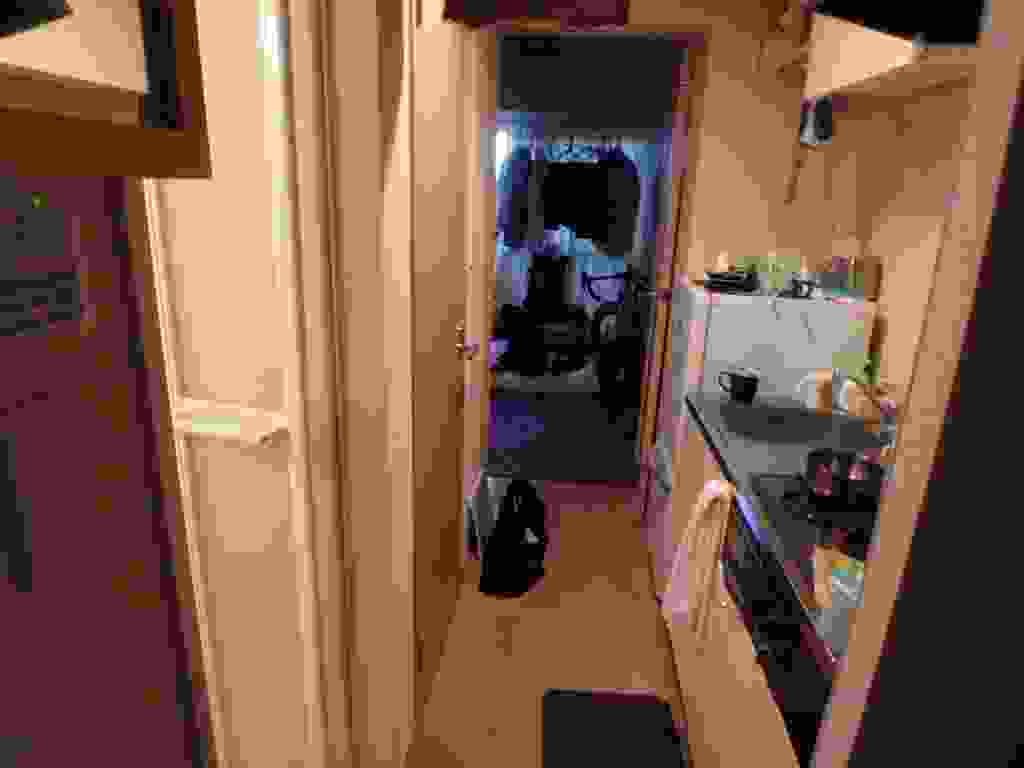
\includegraphics[width=\mywidth]{../wp-content/uploads/2015/07/P7195495-1024x768.jpg} \end{center}

 

 Il a beaucoup voyagé en vélo, en Europe, en Afrique et en Amérique. Maintenant il travaille à Tokyo, de gros horaires, je n'ai pas passé beaucoup de temps avec lui ! 

 

\begin{center} 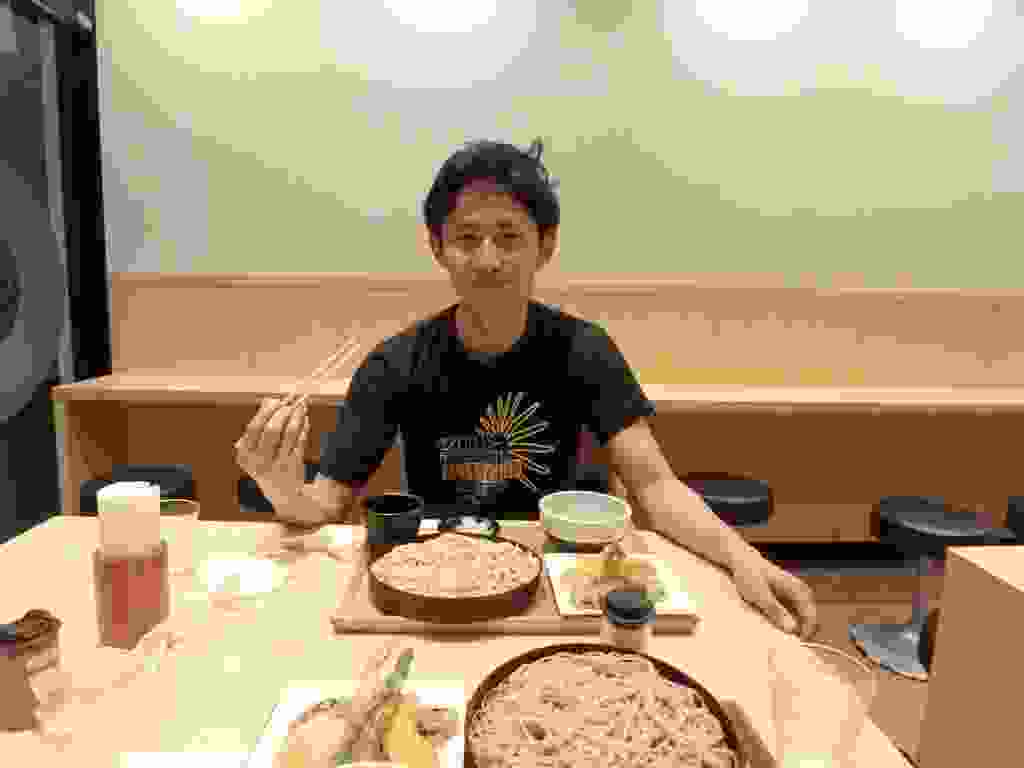
\includegraphics[width=\mywidth]{../wp-content/uploads/2015/07/P7170025-1024x768.jpg} \end{center}

 

 Tokyo est une ville immense avec au moins une dizaine de quartiers intéressants à visiter, chacun avec son ambiance et ses particularités. 

 J'ai commencé par Shinjuku où j'ai acheté un nouvel appareil photo dans un des multiples magasins d'objets électroniques. En plus les magasins au Japon sont tax free pour les étrangers. 

 

\begin{center} 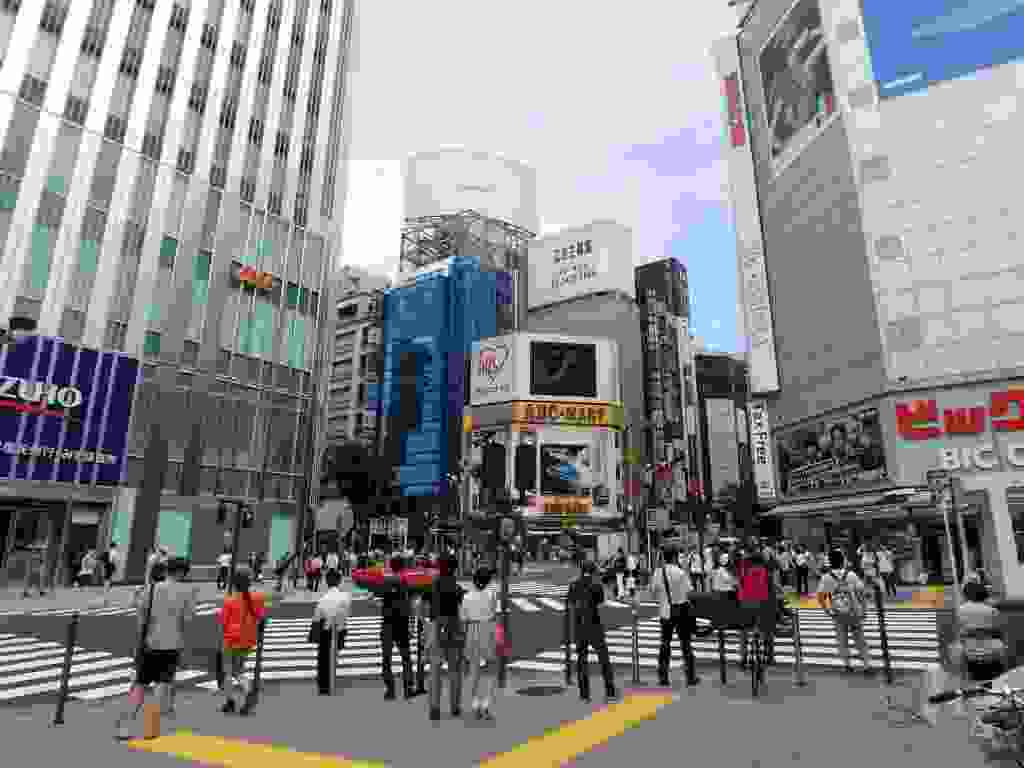
\includegraphics[width=\mywidth]{../wp-content/uploads/2015/07/OI000006-1024x768.jpg} \end{center}

 

 Vue en haut de l'immeuble du Tokyo Metropolitan Government 

 

\begin{center} 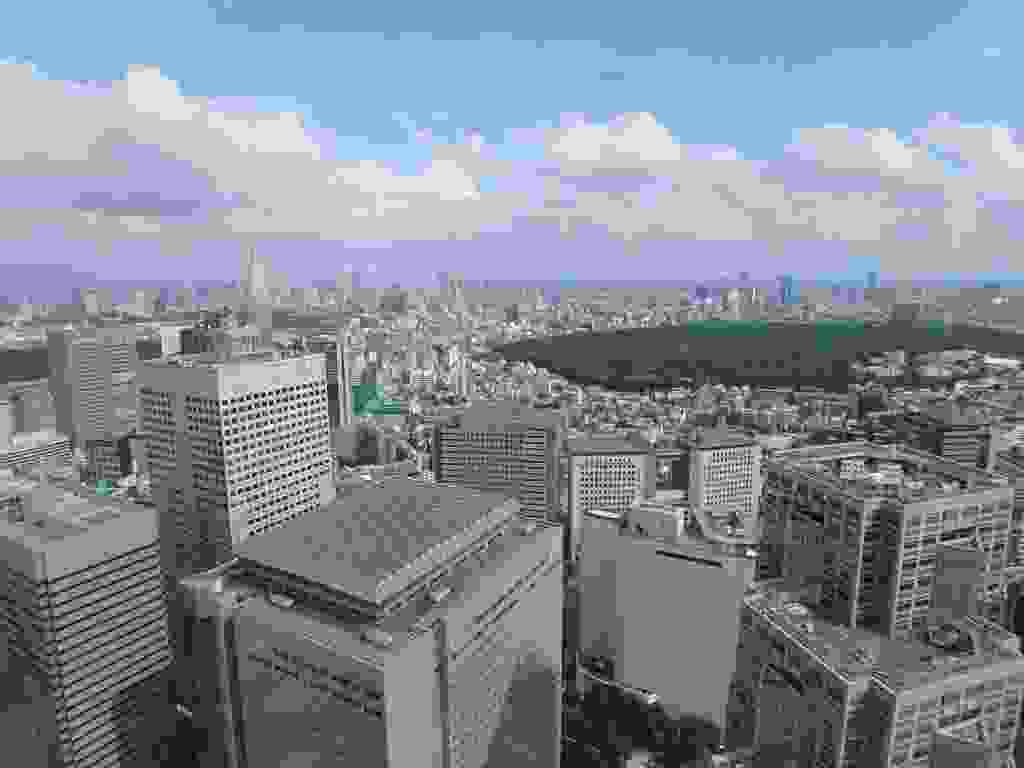
\includegraphics[width=\mywidth]{../wp-content/uploads/2015/07/OI000010-1024x768.jpg} \end{center}

 

 Balade dans le parc Shinjuku Gyoen 

 

\begin{center} 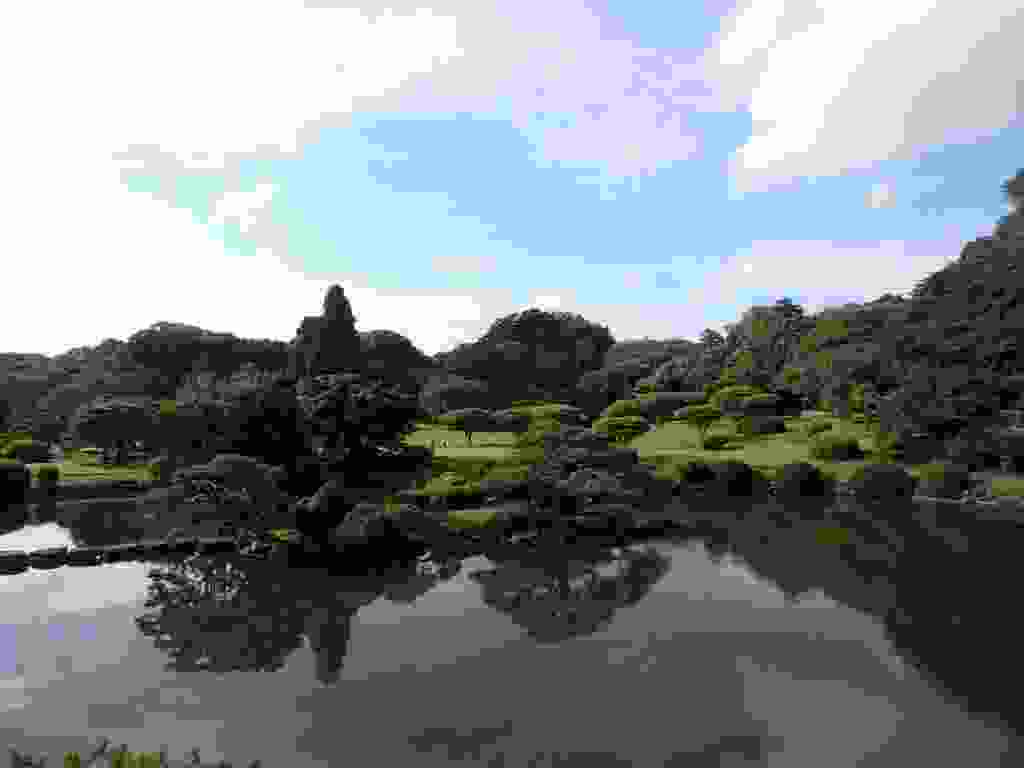
\includegraphics[width=\mywidth]{../wp-content/uploads/2015/07/OI000020-1024x768.jpg} \end{center}

 

 

\begin{center} 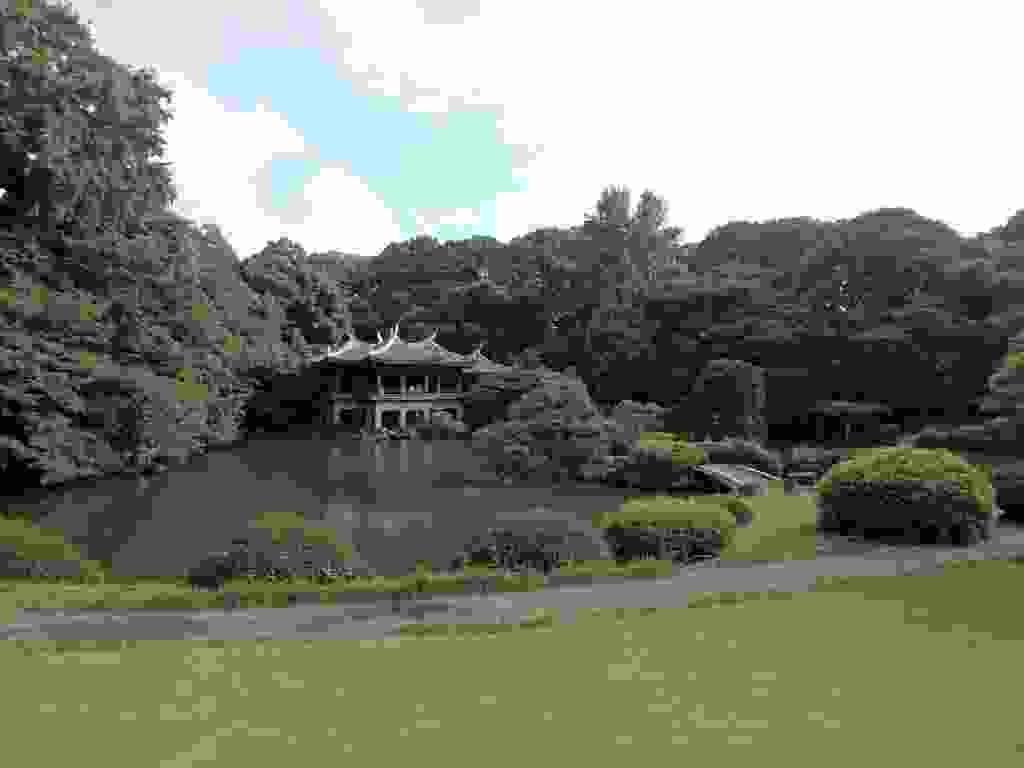
\includegraphics[width=\mywidth]{../wp-content/uploads/2015/07/OI000013-1024x768.jpg} \end{center}

 

 Le petit quartier de Golden Gai Shinjuku : des centaines de minuscules bars regroupés dans 5 ou 6 ruelles. 

 

\begin{center} 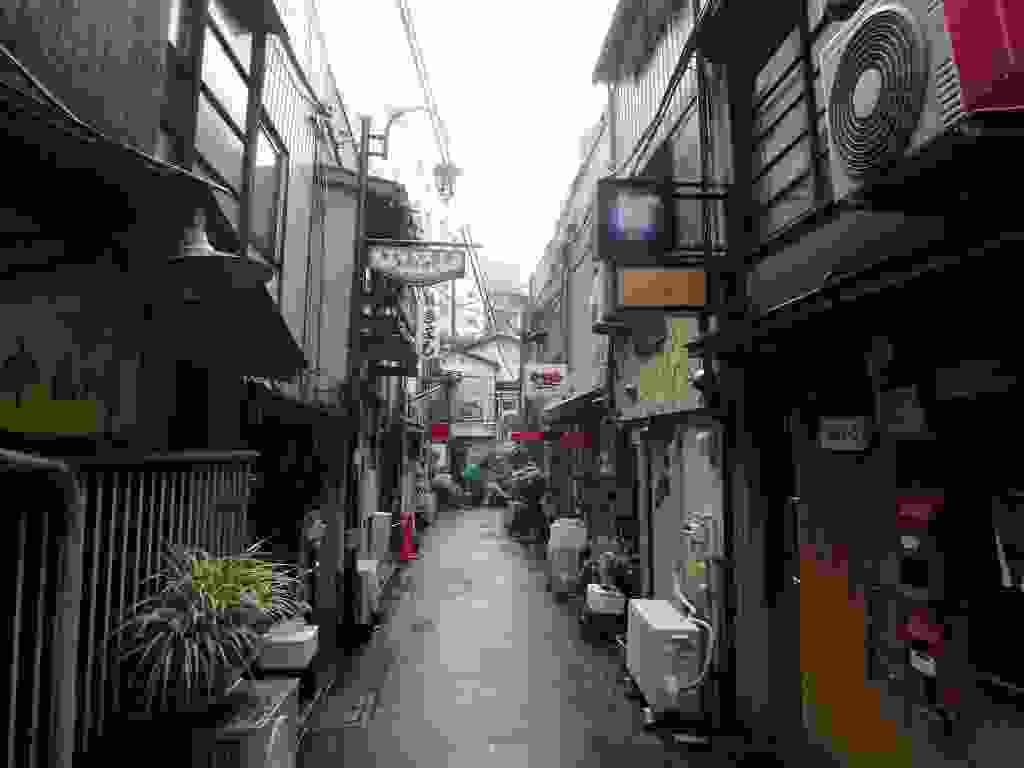
\includegraphics[width=\mywidth]{../wp-content/uploads/2015/07/P7245595-1024x768.jpg} \end{center}

 

 Marunouchi : le quartier central avec le palais impérial et son parc. 

 

\begin{center} 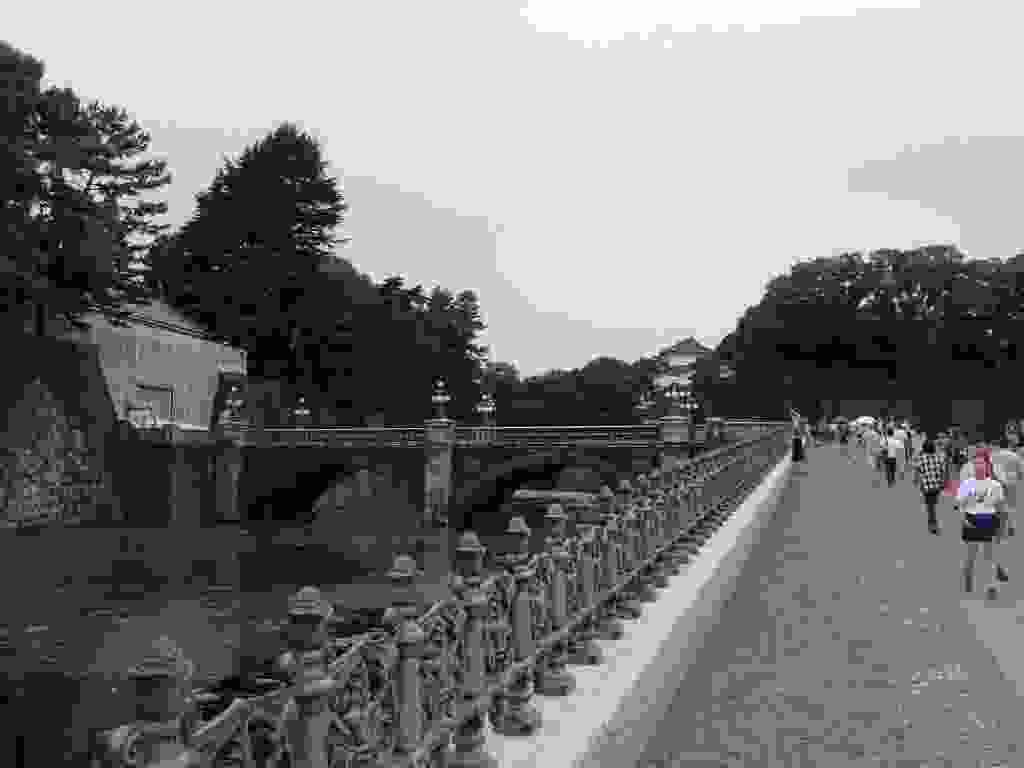
\includegraphics[width=\mywidth]{../wp-content/uploads/2015/07/P7185407-1024x768.jpg} \end{center}

 

 

\begin{center} 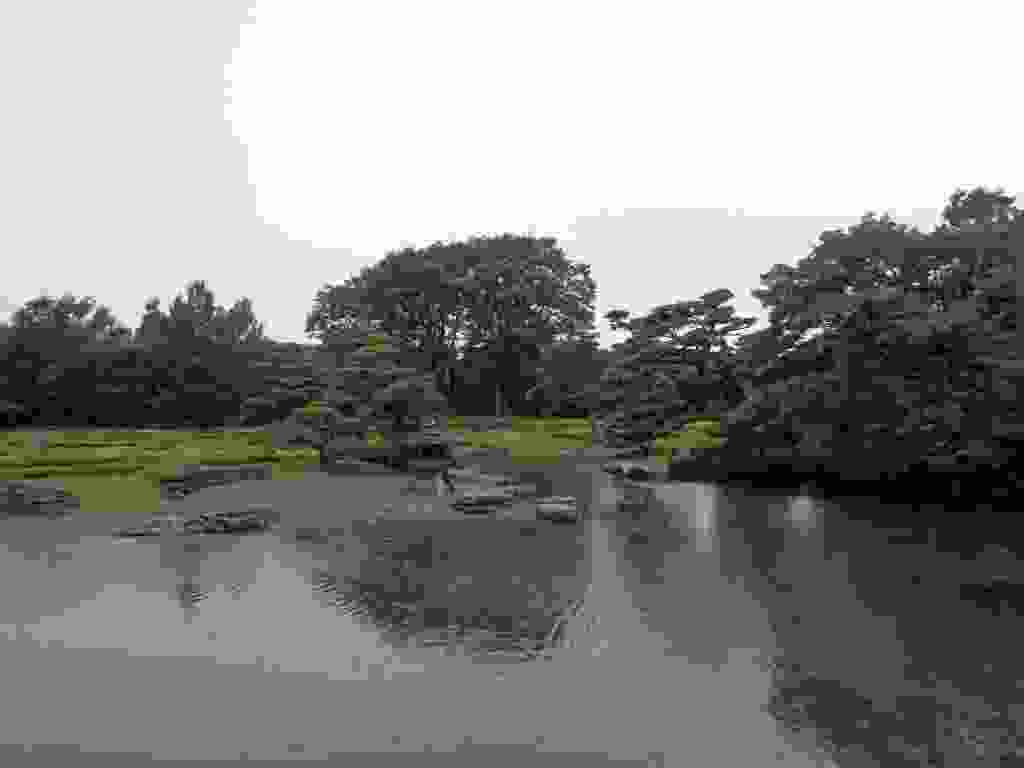
\includegraphics[width=\mywidth]{../wp-content/uploads/2015/07/P7185419-1024x768.jpg} \end{center}

 

 

\begin{center} 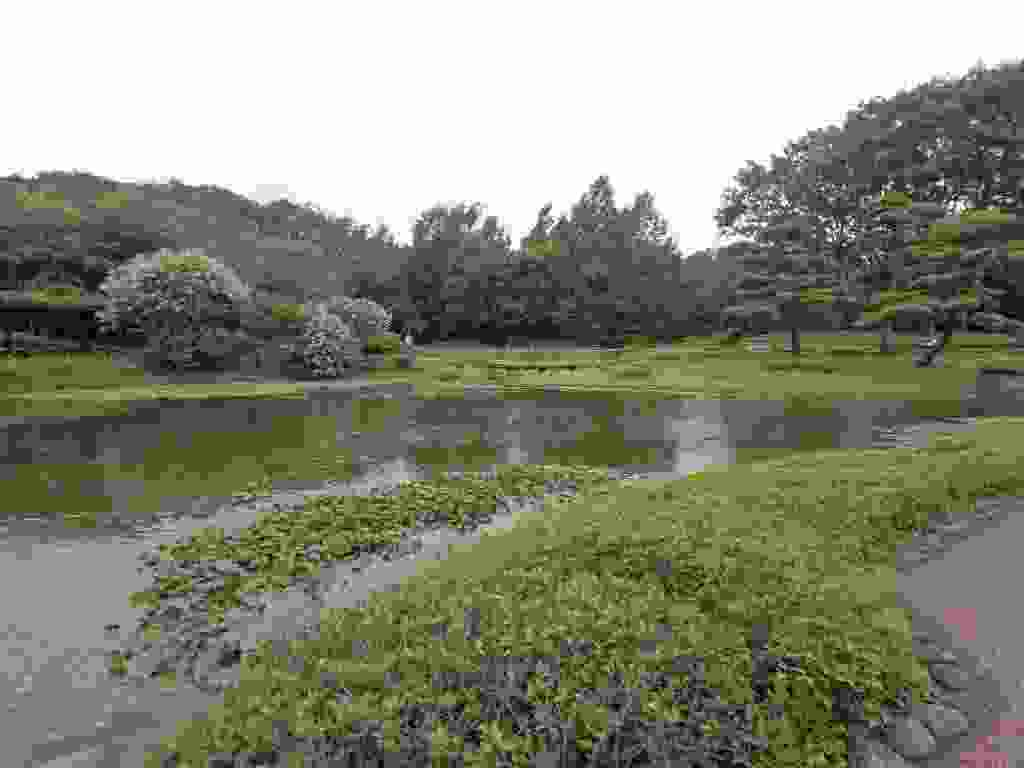
\includegraphics[width=\mywidth]{../wp-content/uploads/2015/07/P7185418-1024x768.jpg} \end{center}

 

 

\begin{center} 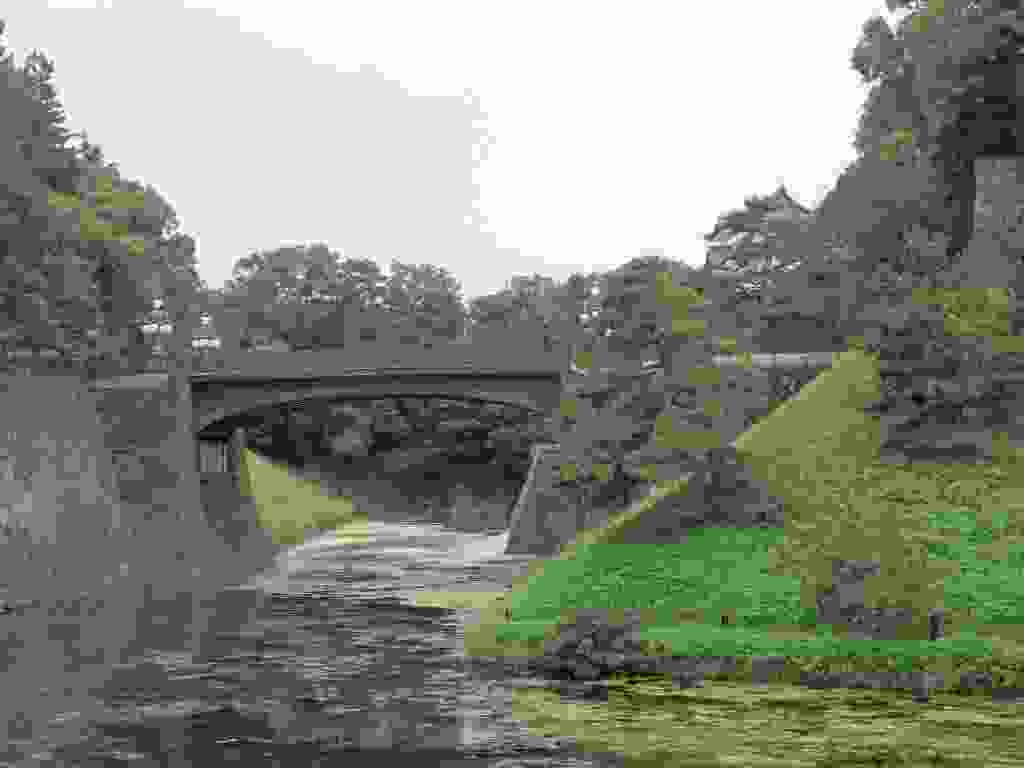
\includegraphics[width=\mywidth]{../wp-content/uploads/2015/07/P7185409-1024x768.jpg} \end{center}

 

 

\begin{center} 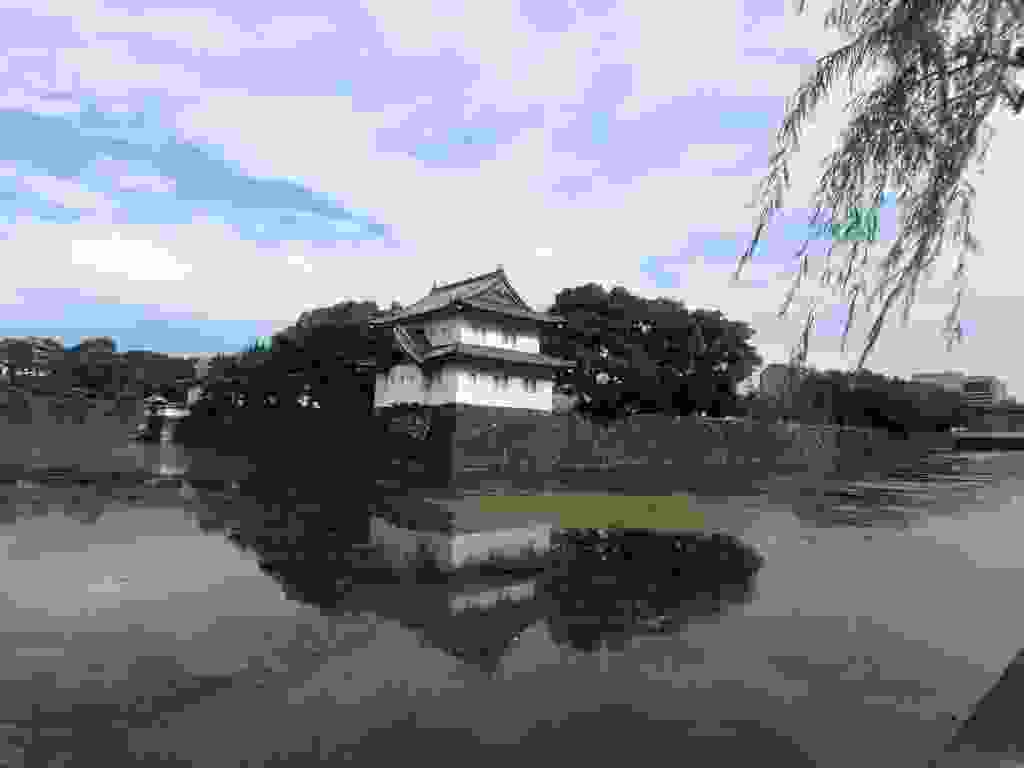
\includegraphics[width=\mywidth]{../wp-content/uploads/2015/07/P7185385-1024x768.jpg} \end{center}

 

 A côté le quartier Ginza et le marché de Tsukiji où on trouve de bons sushis. 

 

\begin{center} 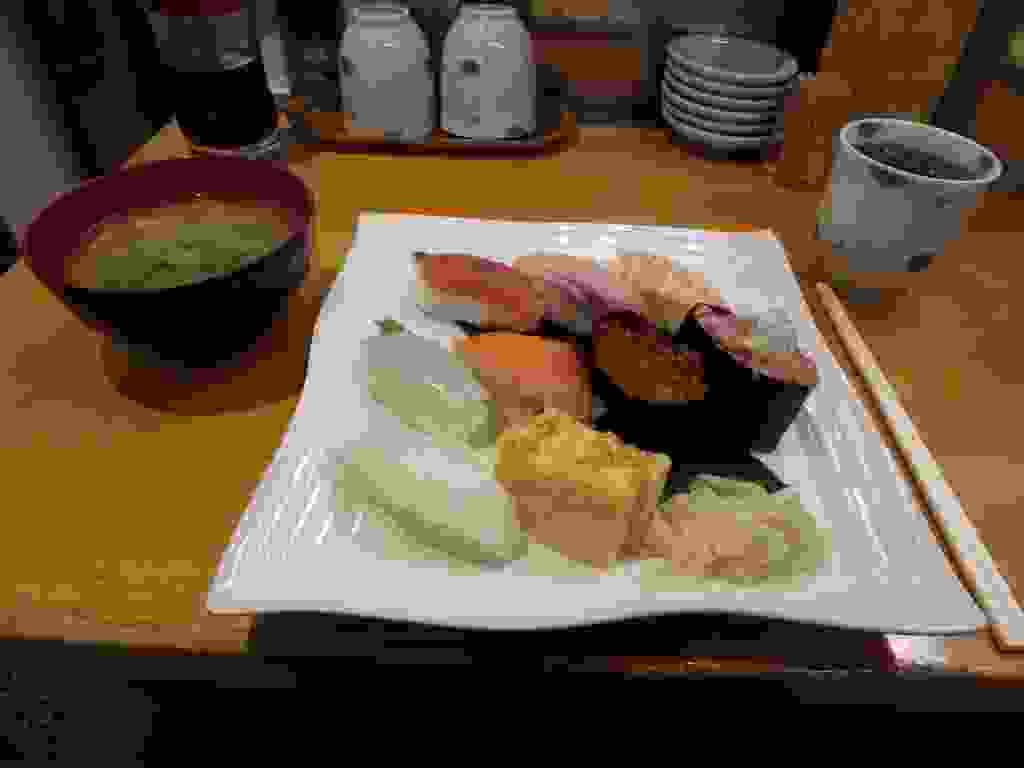
\includegraphics[width=\mywidth]{../wp-content/uploads/2015/07/P7185399-1024x768.jpg} \end{center}

 

 

\begin{center} 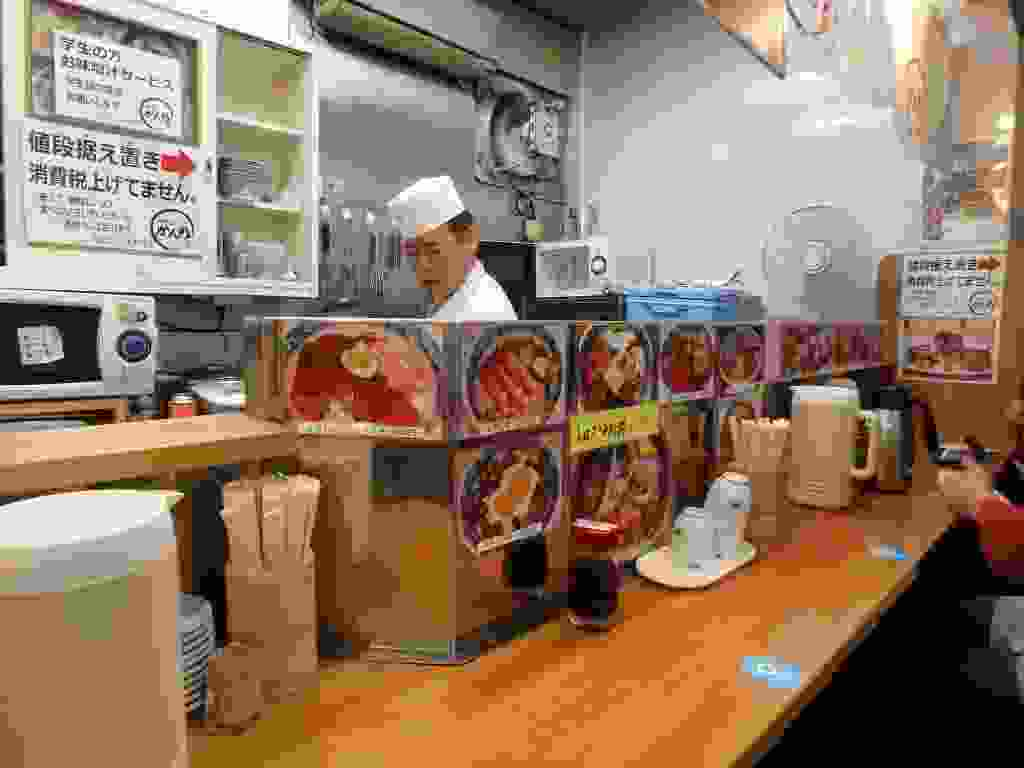
\includegraphics[width=\mywidth]{../wp-content/uploads/2015/07/P7185396-1024x768.jpg} \end{center}

 

 Pour acheter un couteau c'est la aussi 

 

\begin{center} 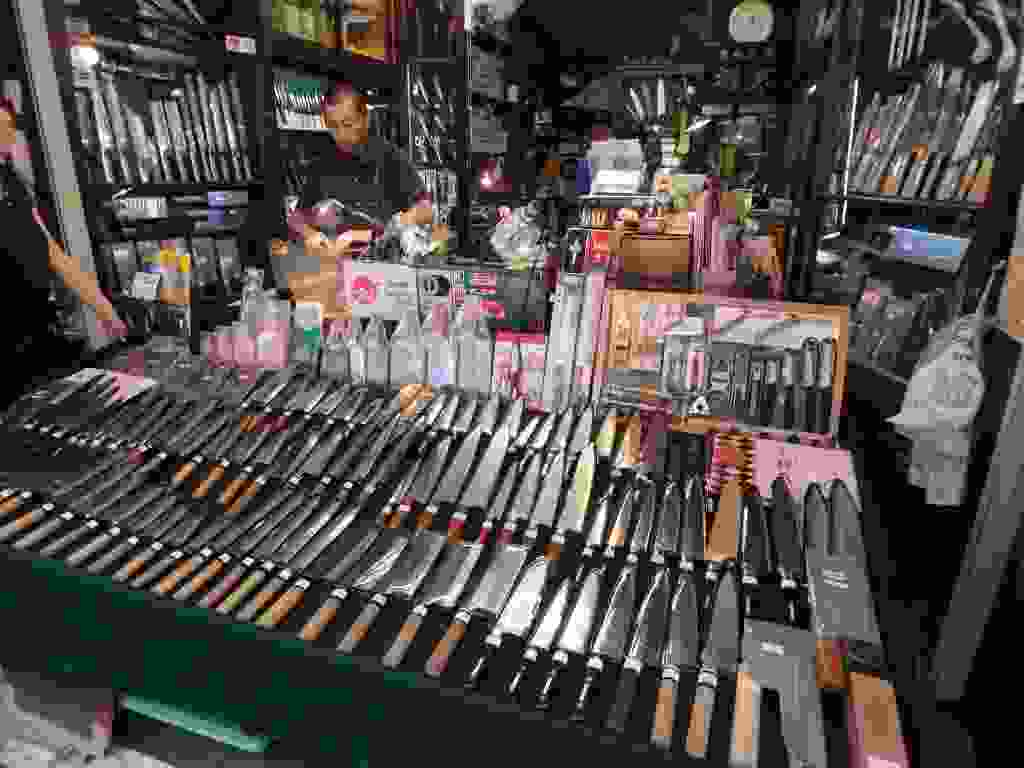
\includegraphics[width=\mywidth]{../wp-content/uploads/2015/07/P7185402-1024x768.jpg} \end{center}

 

 Shibuya : des centres commerciaux immenses et le fameux carrefour avec des passages piétons dans tous les sens. 

 

\begin{center} 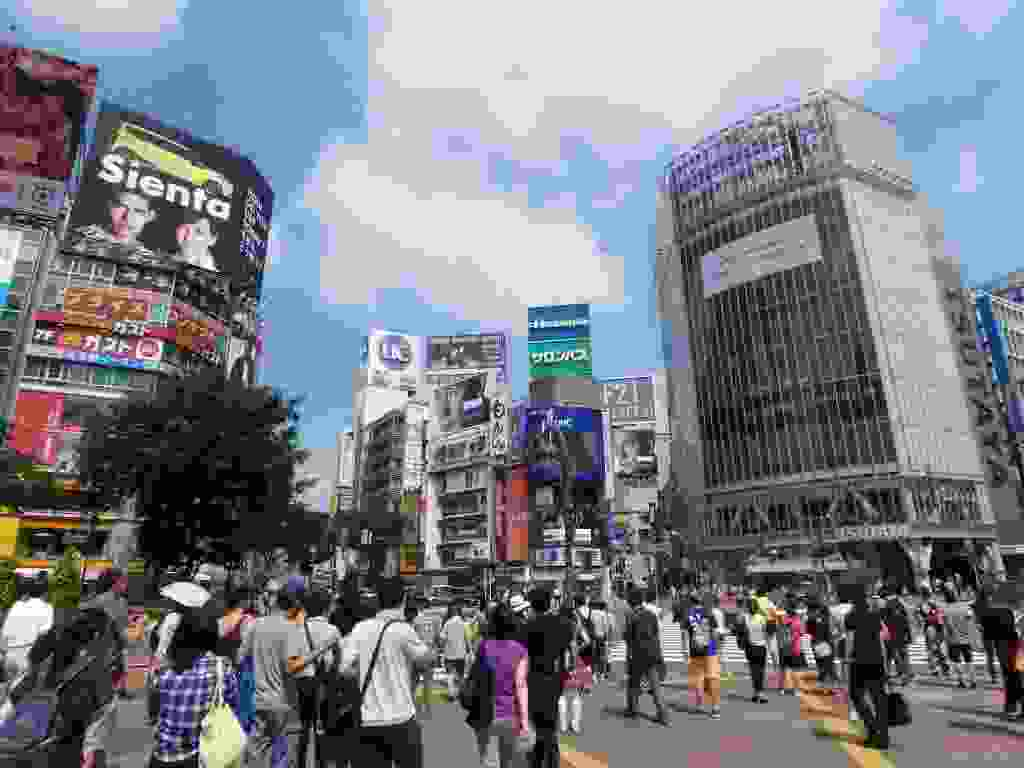
\includegraphics[width=\mywidth]{../wp-content/uploads/2015/07/P7205499-1024x768.jpg} \end{center}

 

 

\begin{center} 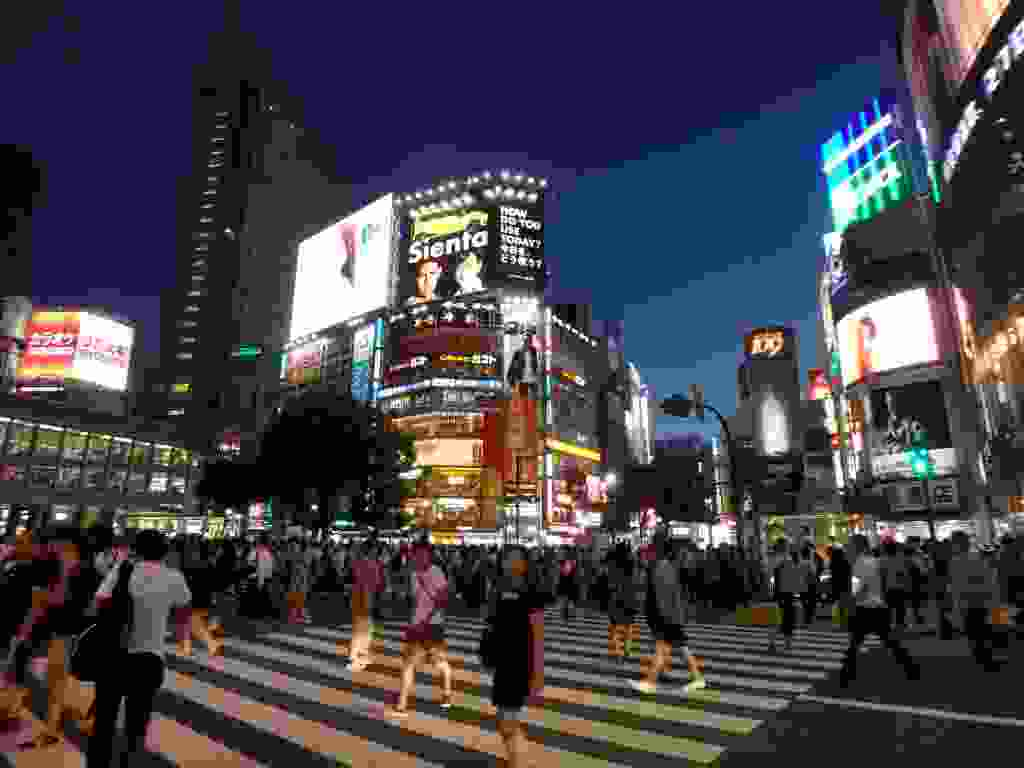
\includegraphics[width=\mywidth]{../wp-content/uploads/2015/07/P7225576-1024x768.jpg} \end{center}

 

 A côté le shrine Meiji Jingu. Au Japon, on trouve soit des temples bouddhistes soit des shrines qui appartiennent à la religion Shinto. 

 

\begin{center} 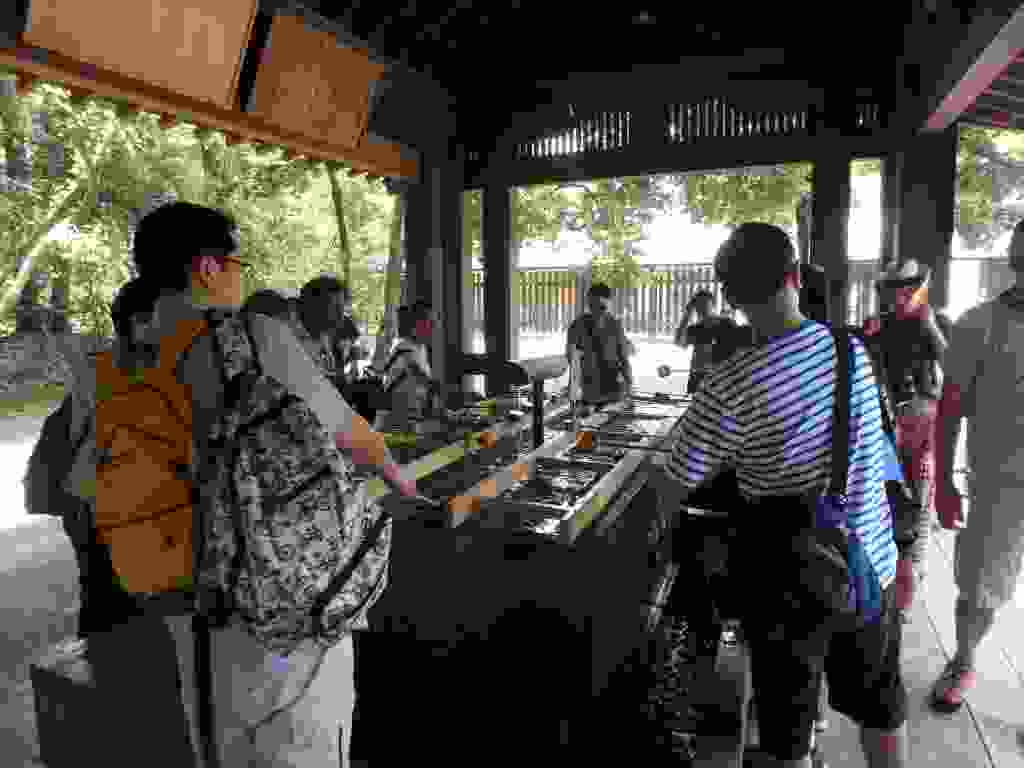
\includegraphics[width=\mywidth]{../wp-content/uploads/2015/07/P7205506-1024x768.jpg} \end{center}

 

 

\begin{center} 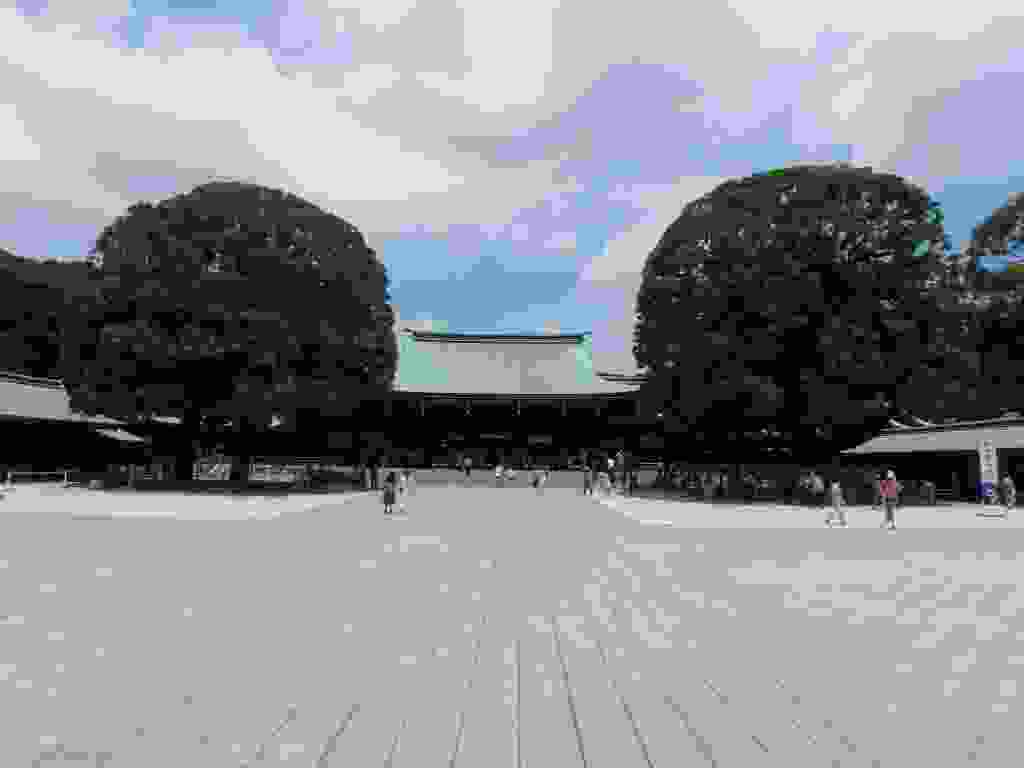
\includegraphics[width=\mywidth]{../wp-content/uploads/2015/07/P7205510-1024x768.jpg} \end{center}

 

 

\begin{center} 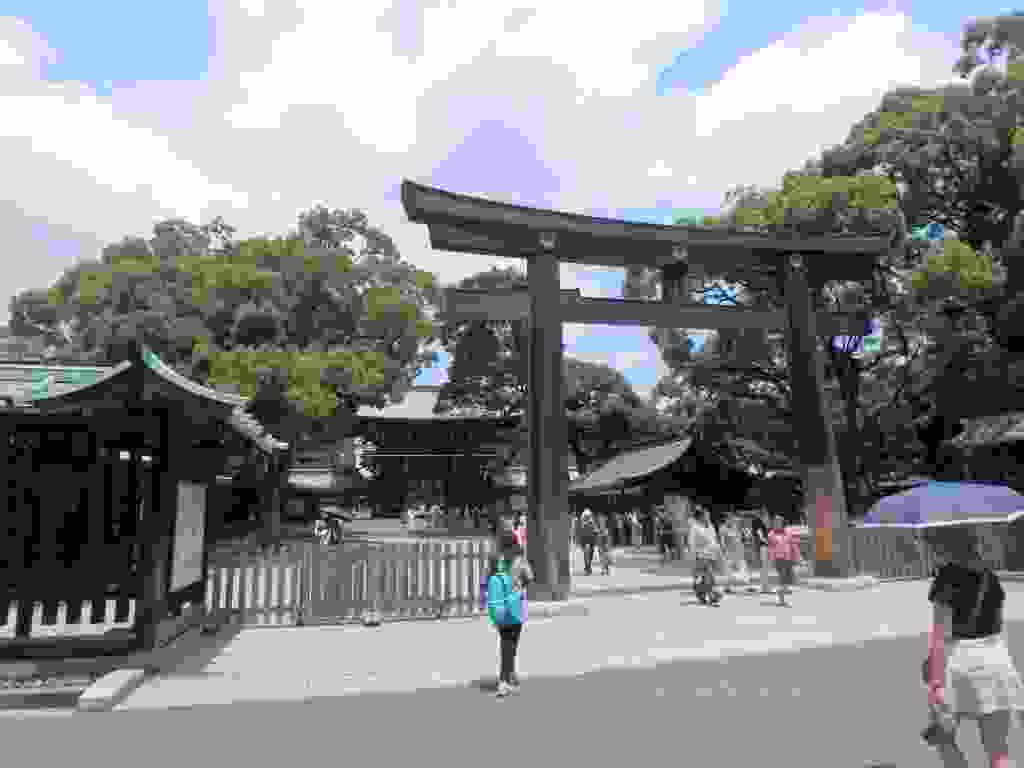
\includegraphics[width=\mywidth]{../wp-content/uploads/2015/07/P7205507-1024x768.jpg} \end{center}

 

 Akihabara et son «electric area», jeux vidéo, manga, maid bar… 

 

\begin{center} 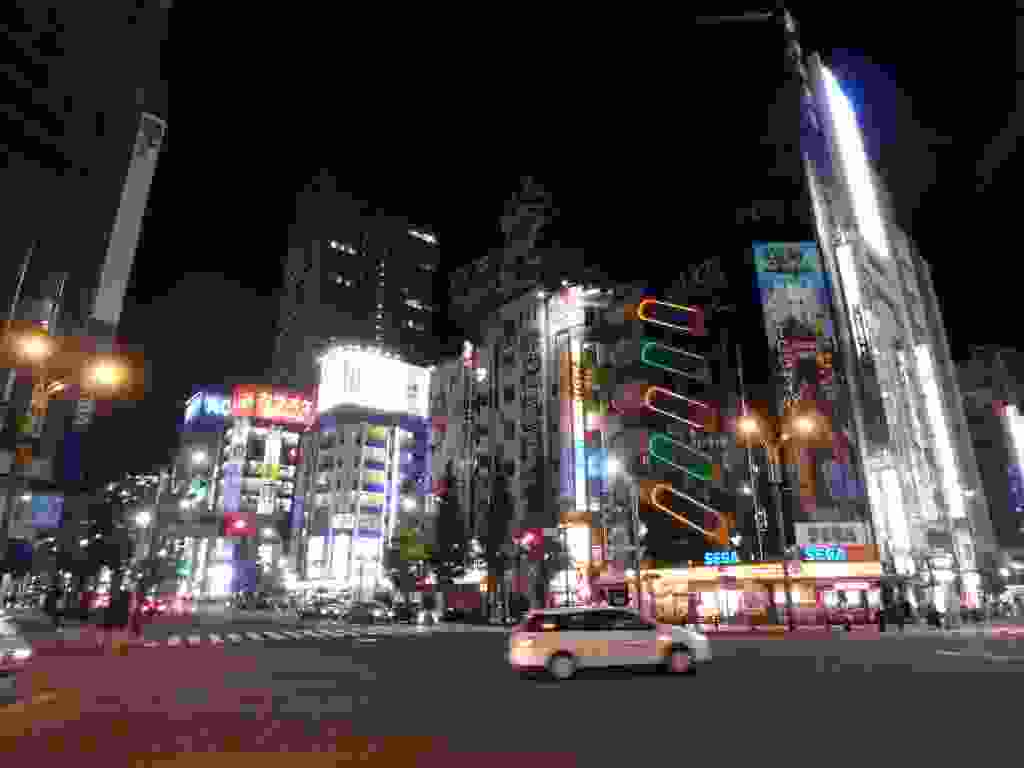
\includegraphics[width=\mywidth]{../wp-content/uploads/2015/07/P7225581-1024x768.jpg} \end{center}

 

 

\begin{center} 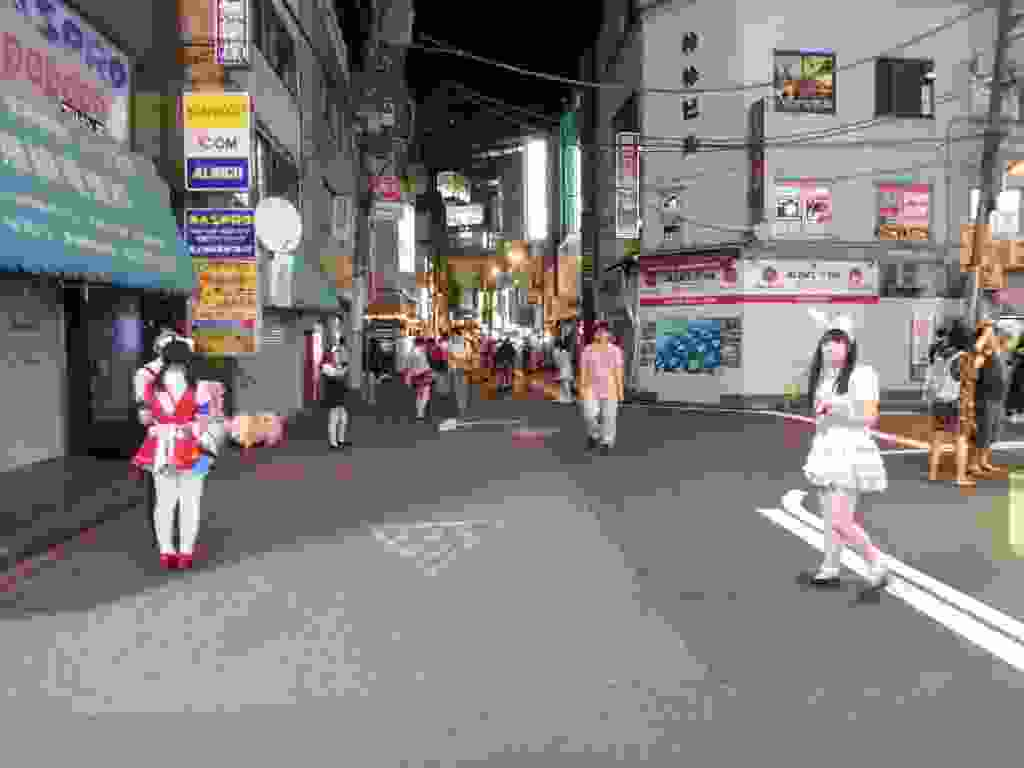
\includegraphics[width=\mywidth]{../wp-content/uploads/2015/07/P7225583-1024x768.jpg} \end{center}

 

 Dans le meme quartier le shrine Yushokan Yasukuni-jinja 

 

\begin{center} 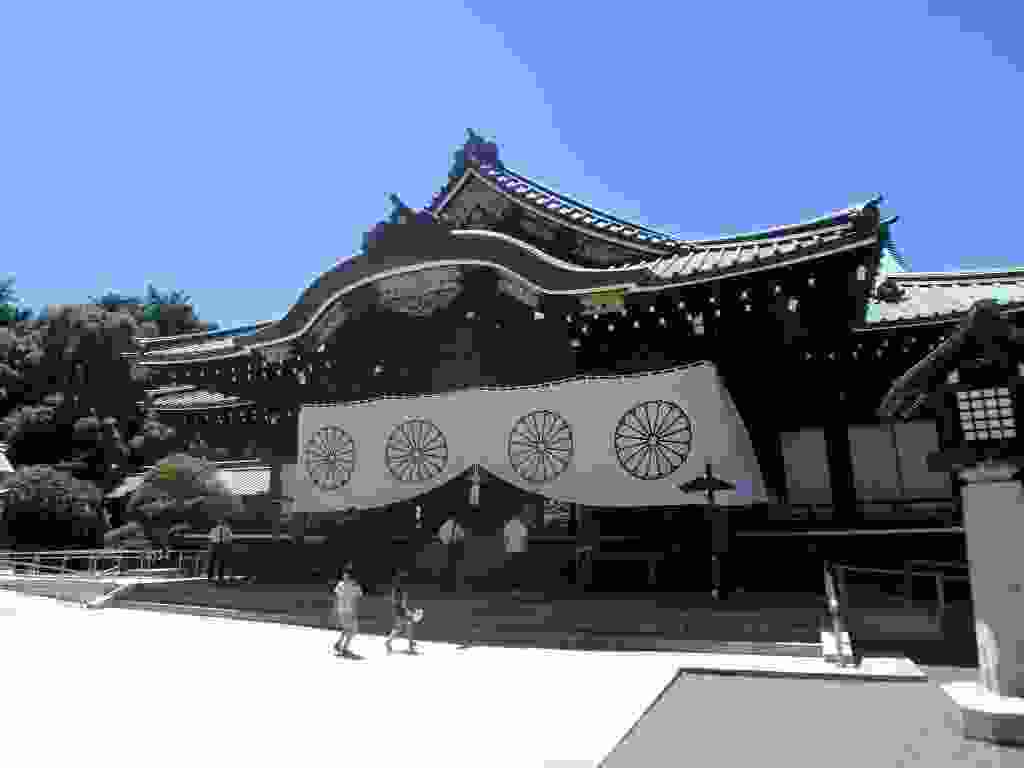
\includegraphics[width=\mywidth]{../wp-content/uploads/2015/07/P7225559-1024x768.jpg} \end{center}

 

 Le quartier Ueno et son grand parc qui contient de beaux temples et shrines. 

 

\begin{center} 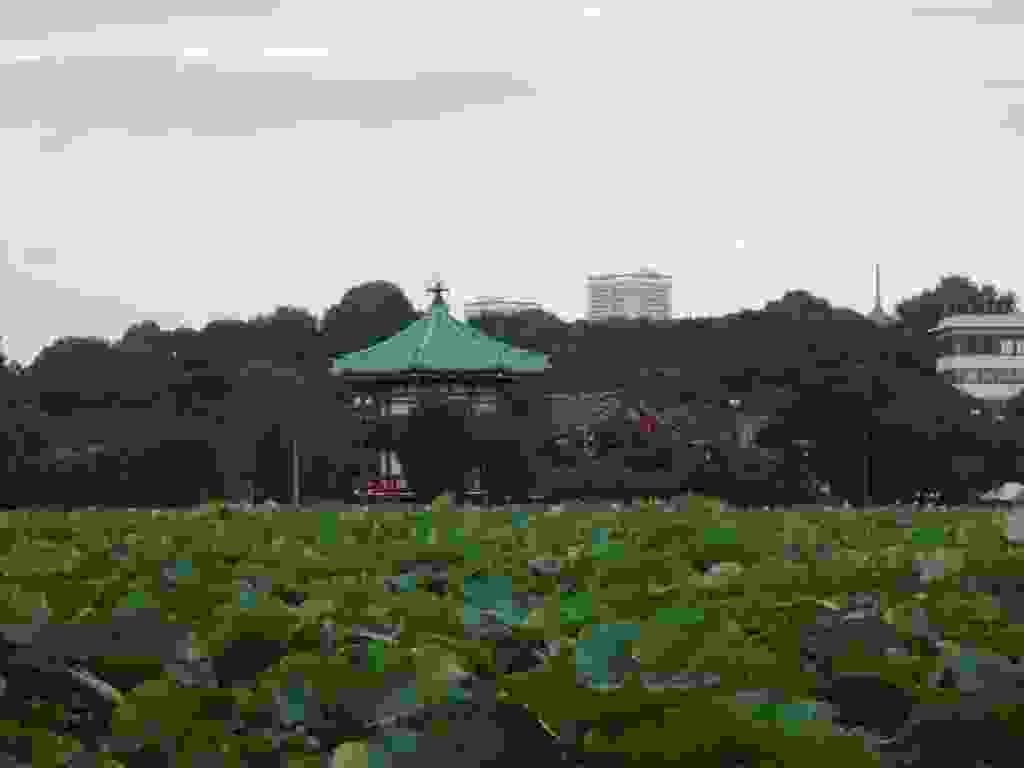
\includegraphics[width=\mywidth]{../wp-content/uploads/2015/07/P7195486-1024x768.jpg} \end{center}

 

 

\begin{center} 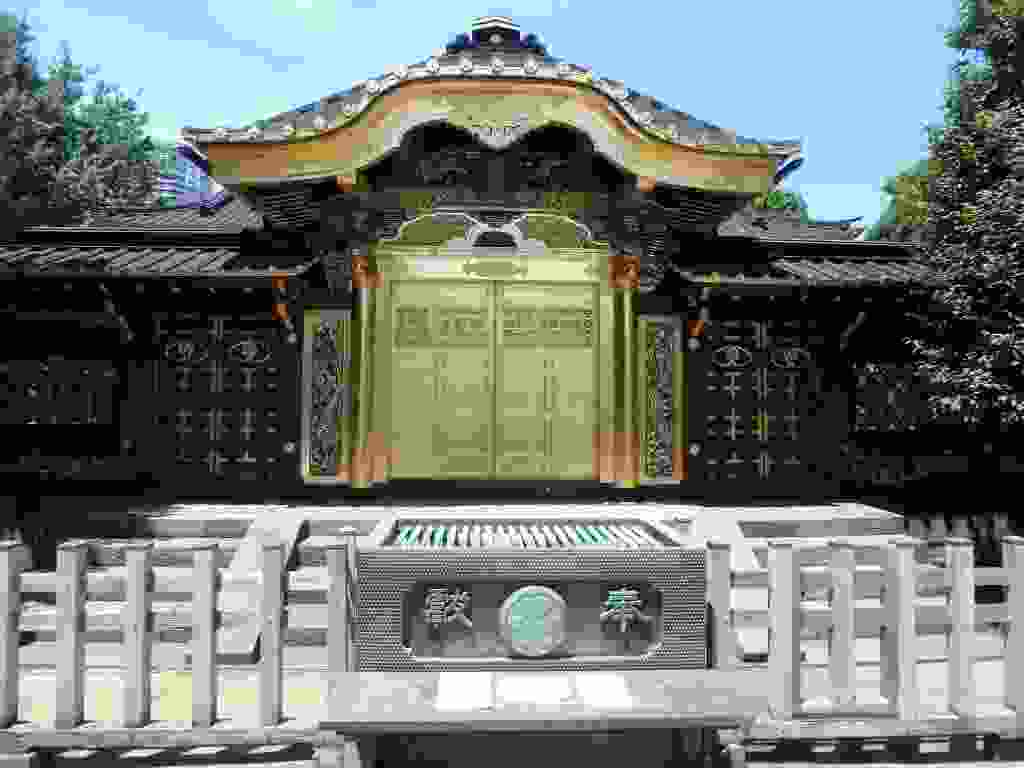
\includegraphics[width=\mywidth]{../wp-content/uploads/2015/07/P7195441-1024x768.jpg} \end{center}

 

 

\begin{center} 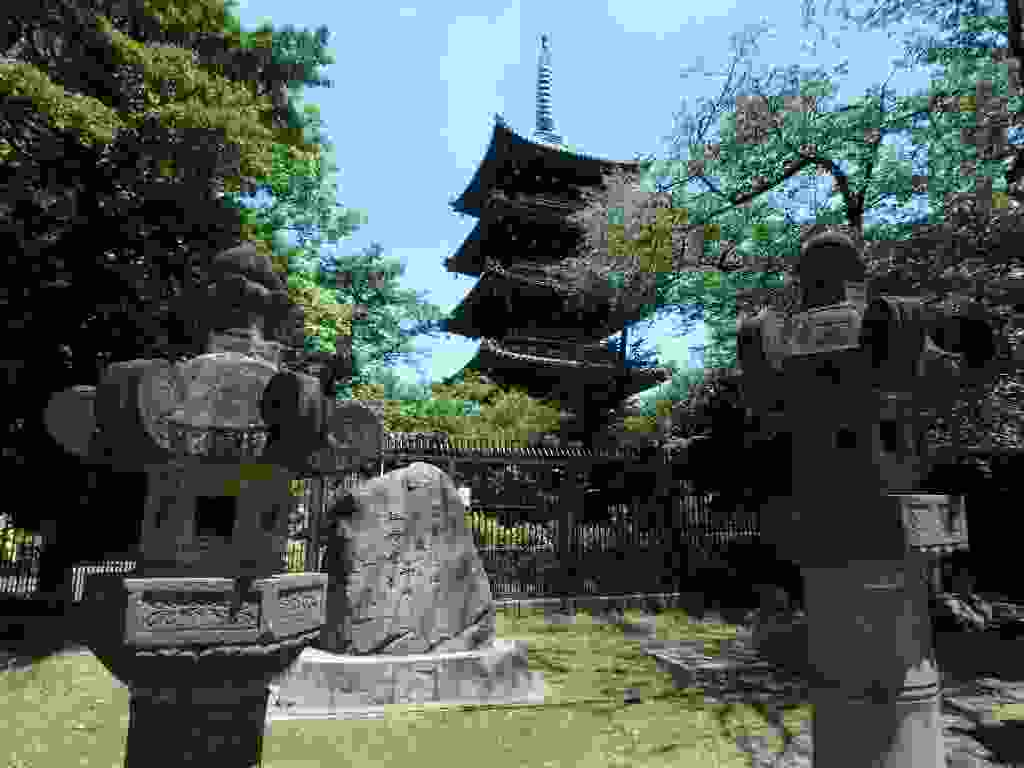
\includegraphics[width=\mywidth]{../wp-content/uploads/2015/07/P7195444-1024x768.jpg} \end{center}

 

 Le temple Kaneiji 

 

\begin{center} 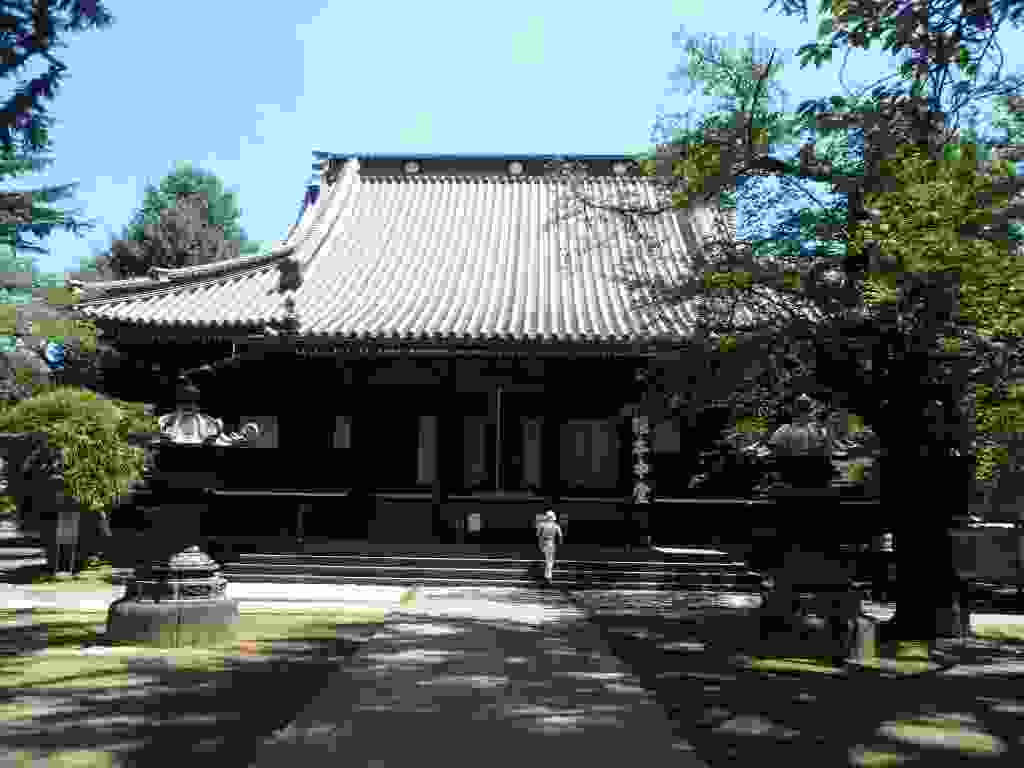
\includegraphics[width=\mywidth]{../wp-content/uploads/2015/07/P7195452-1024x768.jpg} \end{center}

 

 Shrine Yushima Tenmangu 

 

\begin{center} 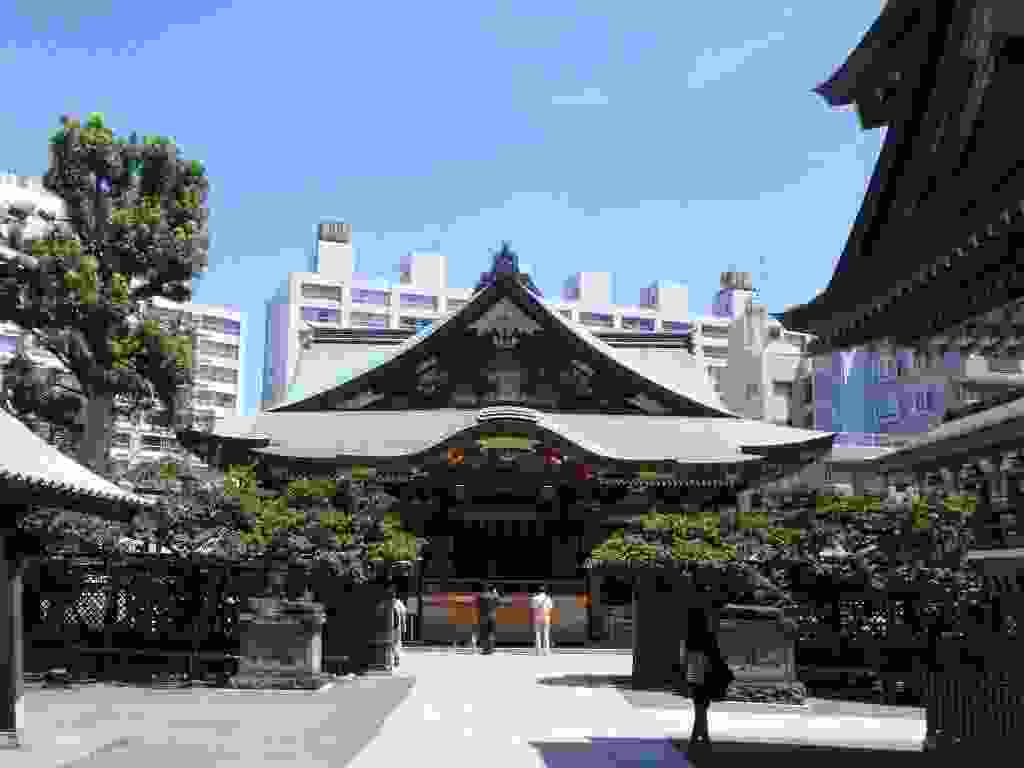
\includegraphics[width=\mywidth]{../wp-content/uploads/2015/07/P7195430-1024x768.jpg} \end{center}

 

 Un peu plus loin, le quartier Asakusa 

 La rue commerçante Nakamise, l'alignement de boutiques date de l'époque d'Edo (ancien nom de Tokyo). 

 

\begin{center} 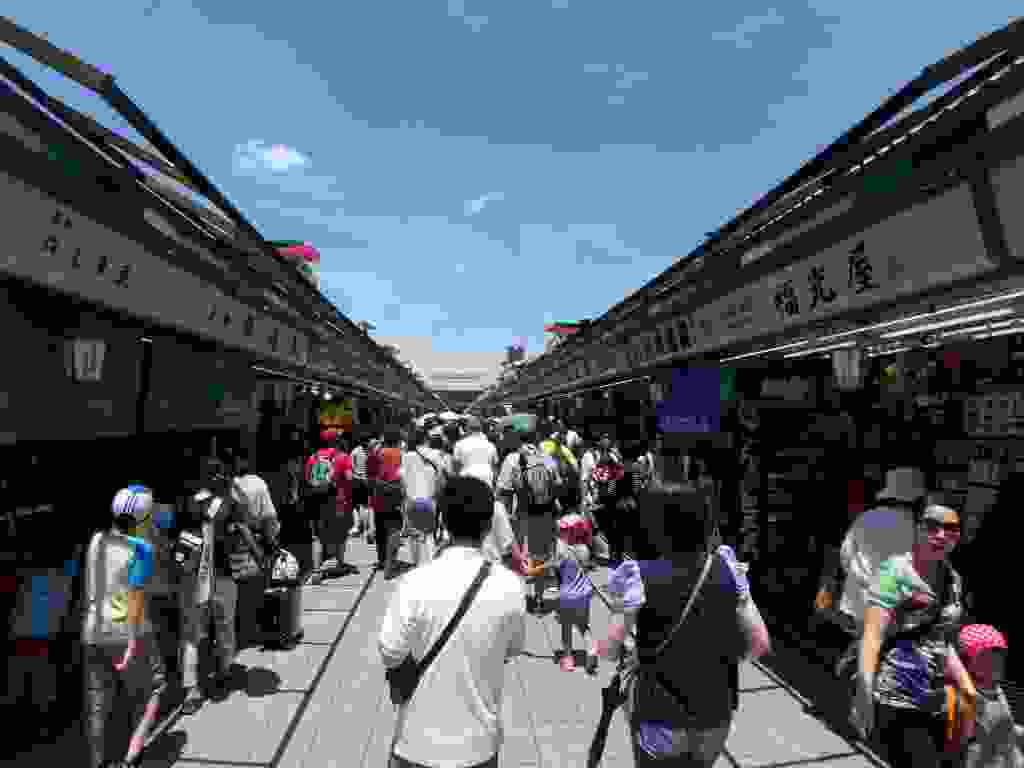
\includegraphics[width=\mywidth]{../wp-content/uploads/2015/07/P7195457-1024x768.jpg} \end{center}

 

 Le célèbre Temple Sensoji 

 

\begin{center} 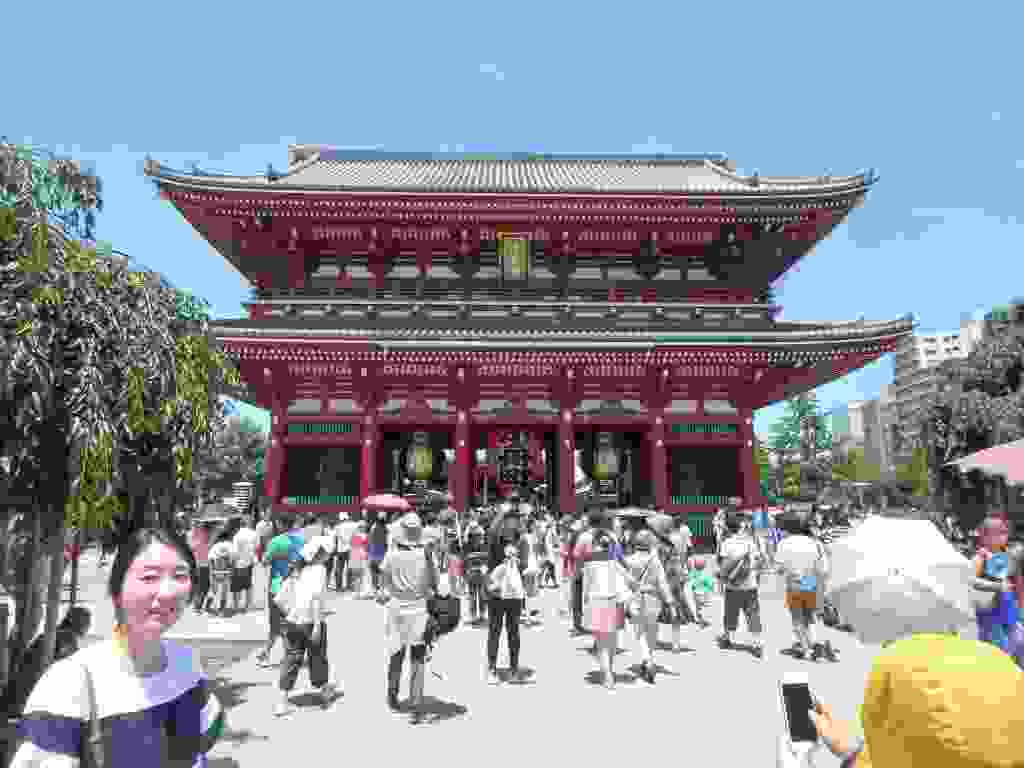
\includegraphics[width=\mywidth]{../wp-content/uploads/2015/07/P7195458-1024x768.jpg} \end{center}

 

 

\begin{center} 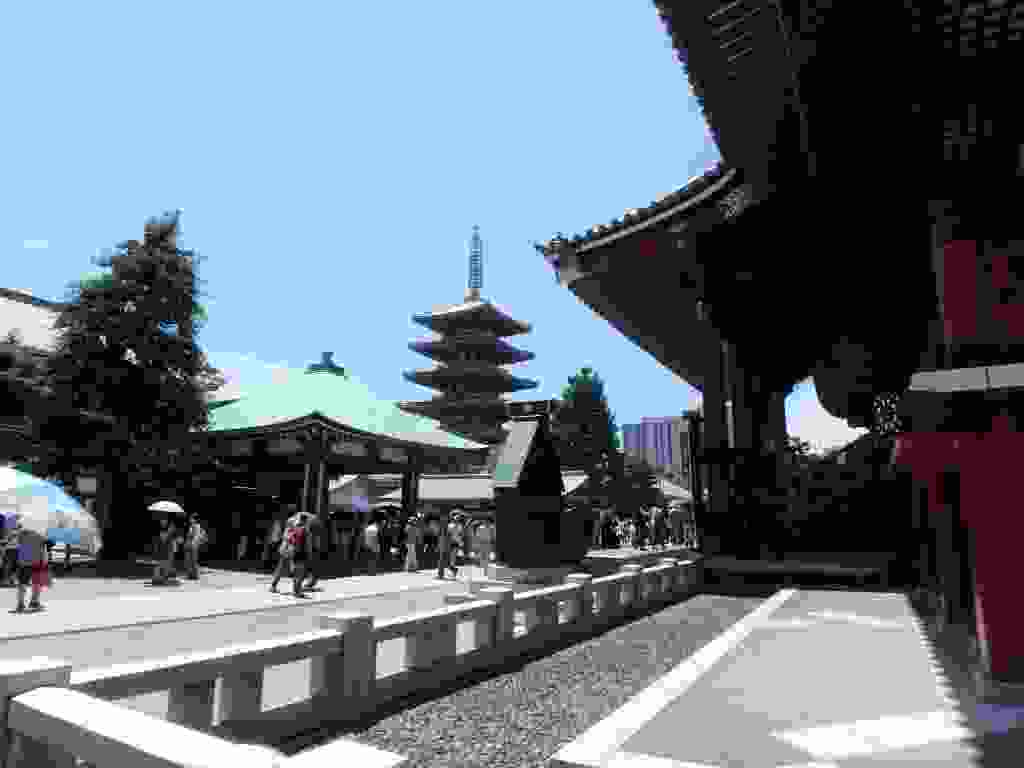
\includegraphics[width=\mywidth]{../wp-content/uploads/2015/07/P7195466-1024x768.jpg} \end{center}

 

 

\begin{center} 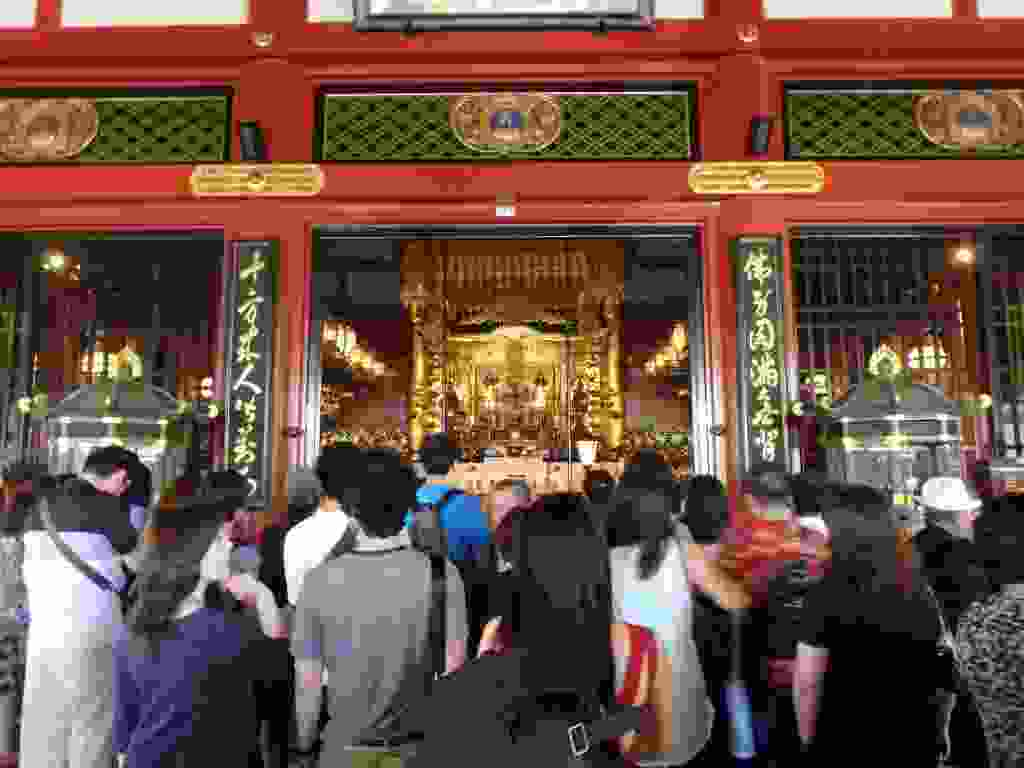
\includegraphics[width=\mywidth]{../wp-content/uploads/2015/07/P7195464-1024x768.jpg} \end{center}

 

 La tour Skytree 

 

\begin{center} 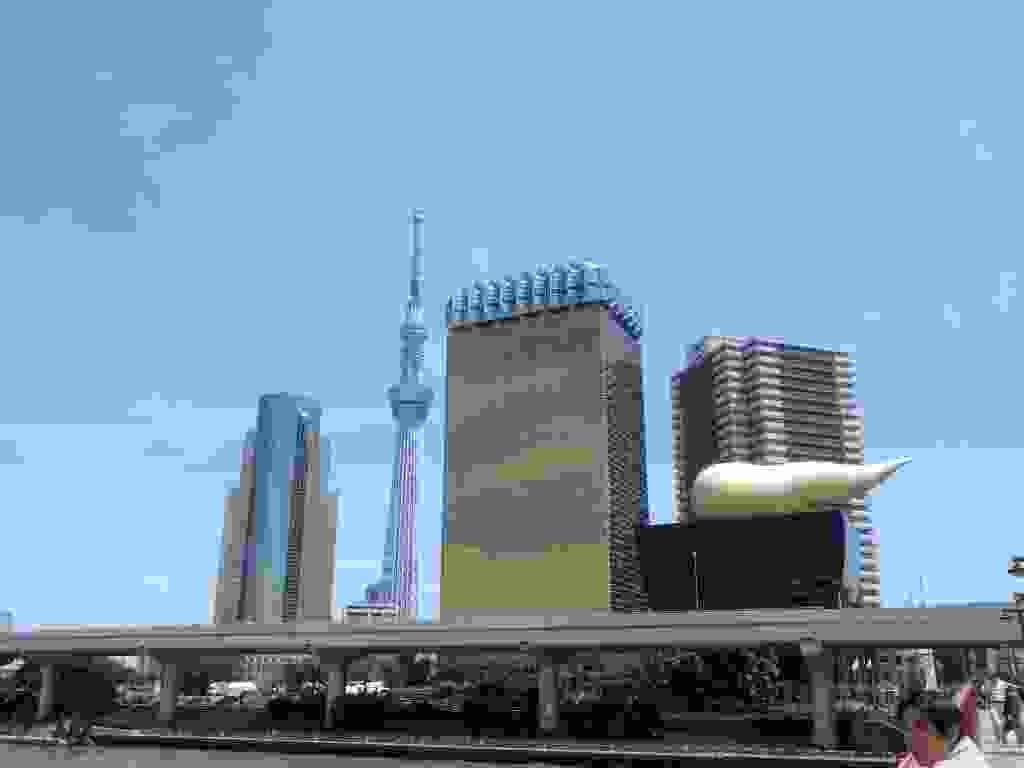
\includegraphics[width=\mywidth]{../wp-content/uploads/2015/07/P7195472-1024x768.jpg} \end{center}

 

 Je me suis déplacé la plupart du temps en vélo mais j'ai quand même testé une fois le métro, je m'attendais à ce qu'il soit plus bondé ! 

 

\begin{center} 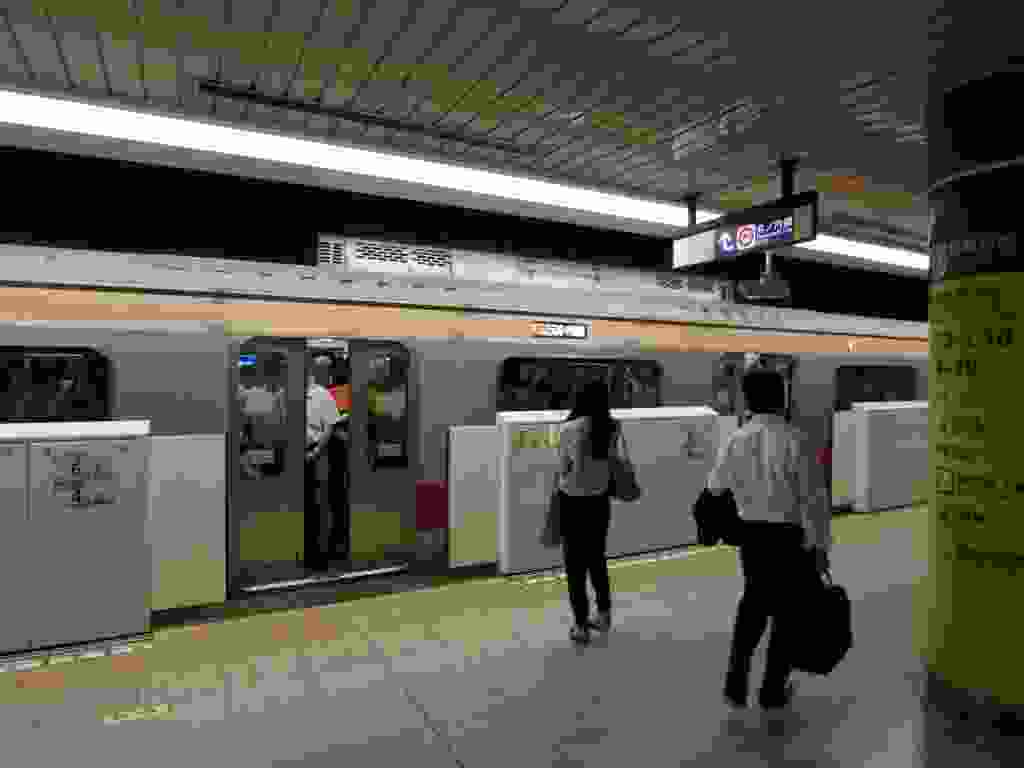
\includegraphics[width=\mywidth]{../wp-content/uploads/2015/07/P7215527-1024x768.jpg} \end{center}

 

 

\begin{center} 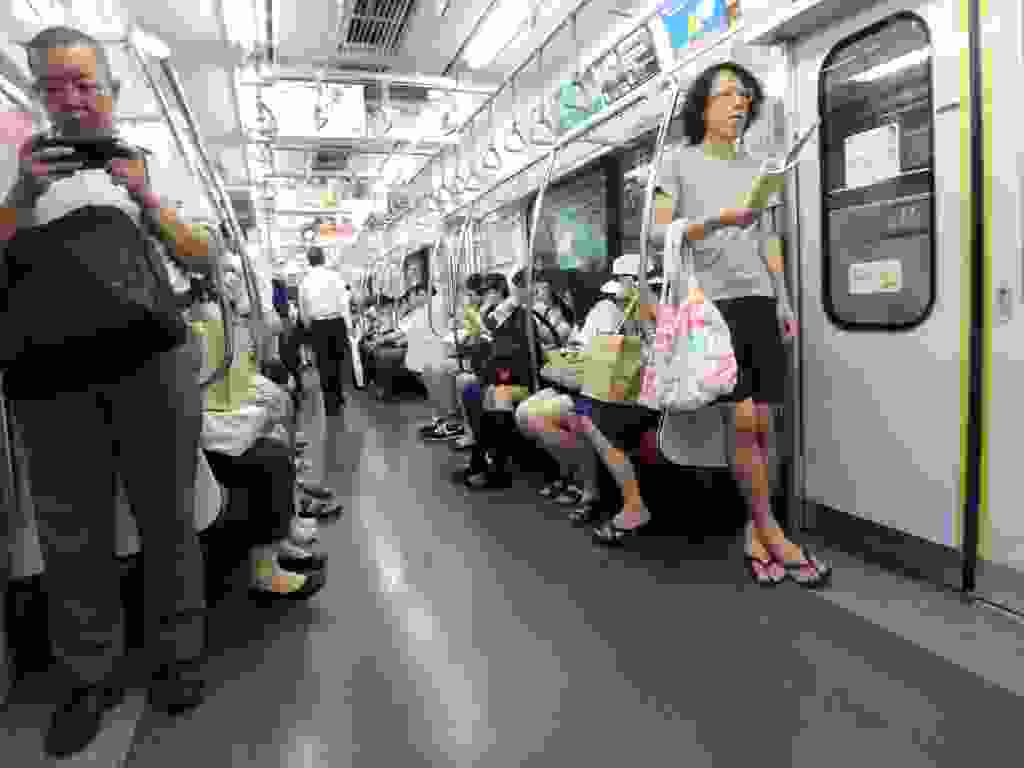
\includegraphics[width=\mywidth]{../wp-content/uploads/2015/07/P7215528-1024x768.jpg} \end{center}

 

 Je me suis arrêté une nuit dans le quartier Ikebukuro pour tester un hôtel capsule : tout le confort necessaire est la ! 

 

\begin{center} 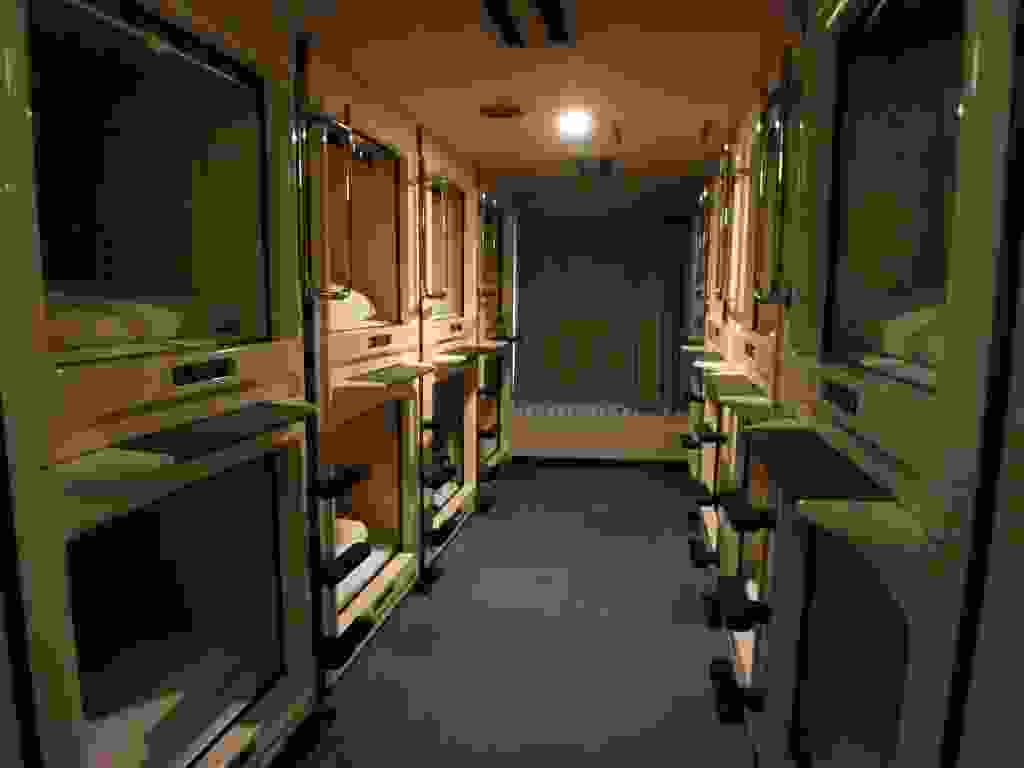
\includegraphics[width=\mywidth]{../wp-content/uploads/2015/07/P7205520-1024x768.jpg} \end{center}

 

 

\begin{center} 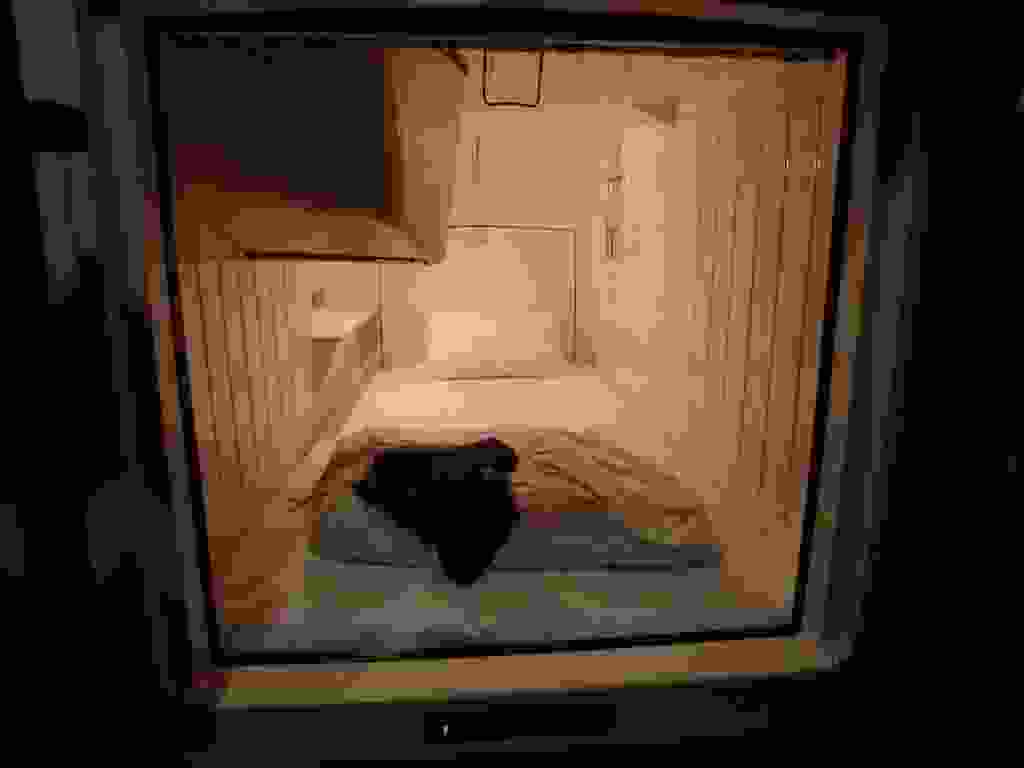
\includegraphics[width=\mywidth]{../wp-content/uploads/2015/07/P7205523-1024x768.jpg} \end{center}

 

 J'ai ensuite été accueilli par Yukiko et Carlos dans leur bel appartement de style japonais. Yukiko est guide pour des visites touristiques de Tokyo en vélo. 

 

\begin{center} 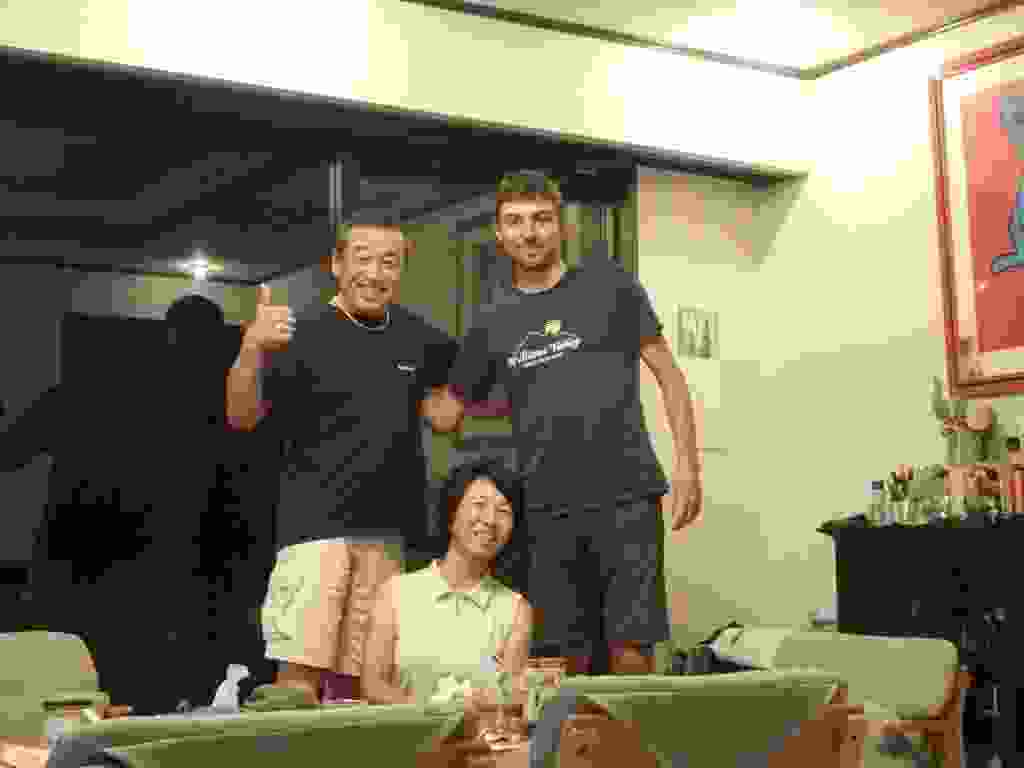
\includegraphics[width=\mywidth]{../wp-content/uploads/2015/07/P7235588-1024x768.jpg} \end{center}

 

 

\begin{center} 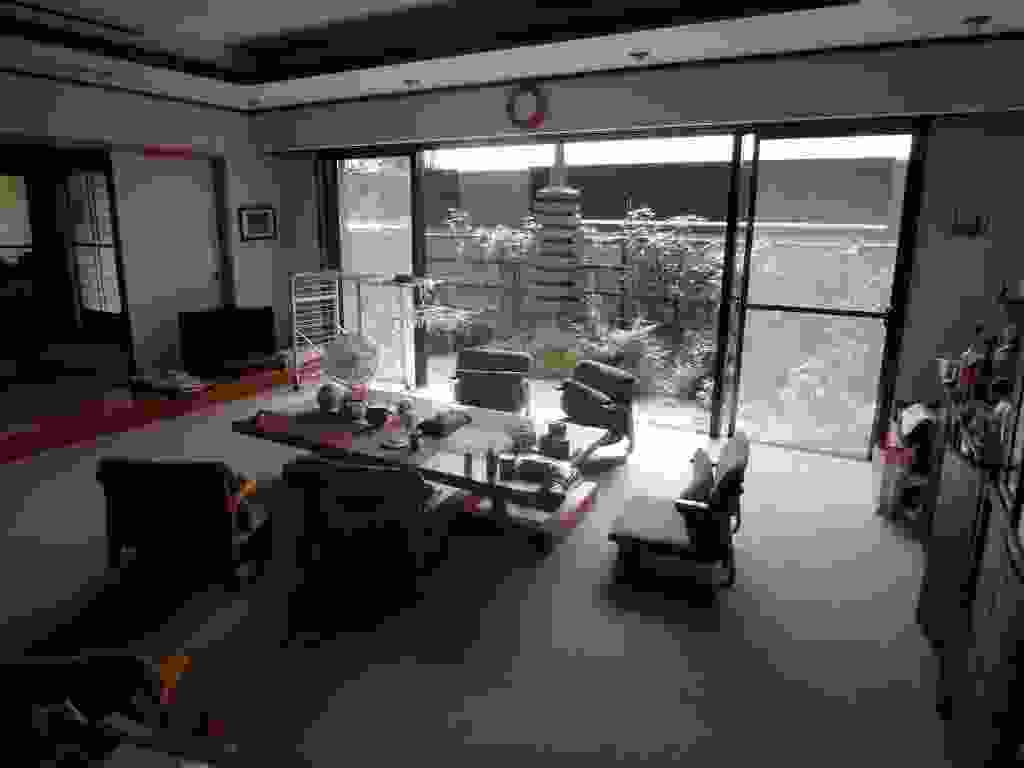
\includegraphics[width=\mywidth]{../wp-content/uploads/2015/07/P7225549-1024x768.jpg} \end{center}

 

 Ils habitent dans le quartier de Kagurazaka. Il y avait un festival avec un défilé, beaucoup de japonais portent un costume traditionnel. 

 

\begin{center} 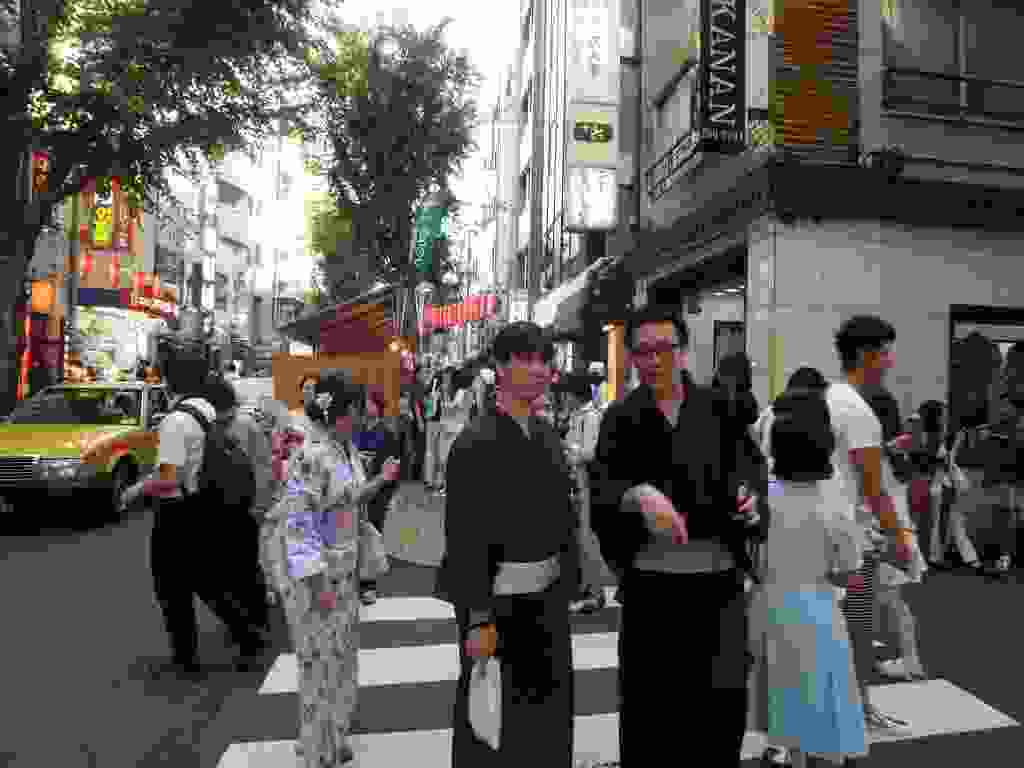
\includegraphics[width=\mywidth]{../wp-content/uploads/2015/07/P7235587-1024x768.jpg} \end{center}

 

 

\begin{center} 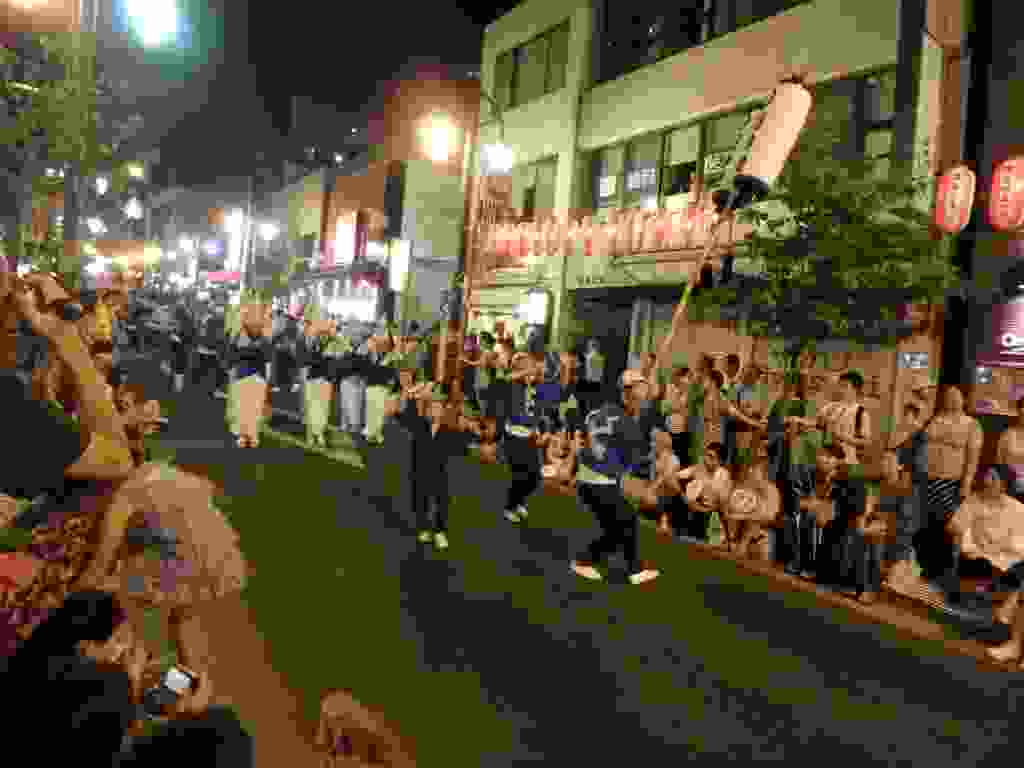
\includegraphics[width=\mywidth]{../wp-content/uploads/2015/07/P7245604-1024x768.jpg} \end{center}

 

 

\begin{center} 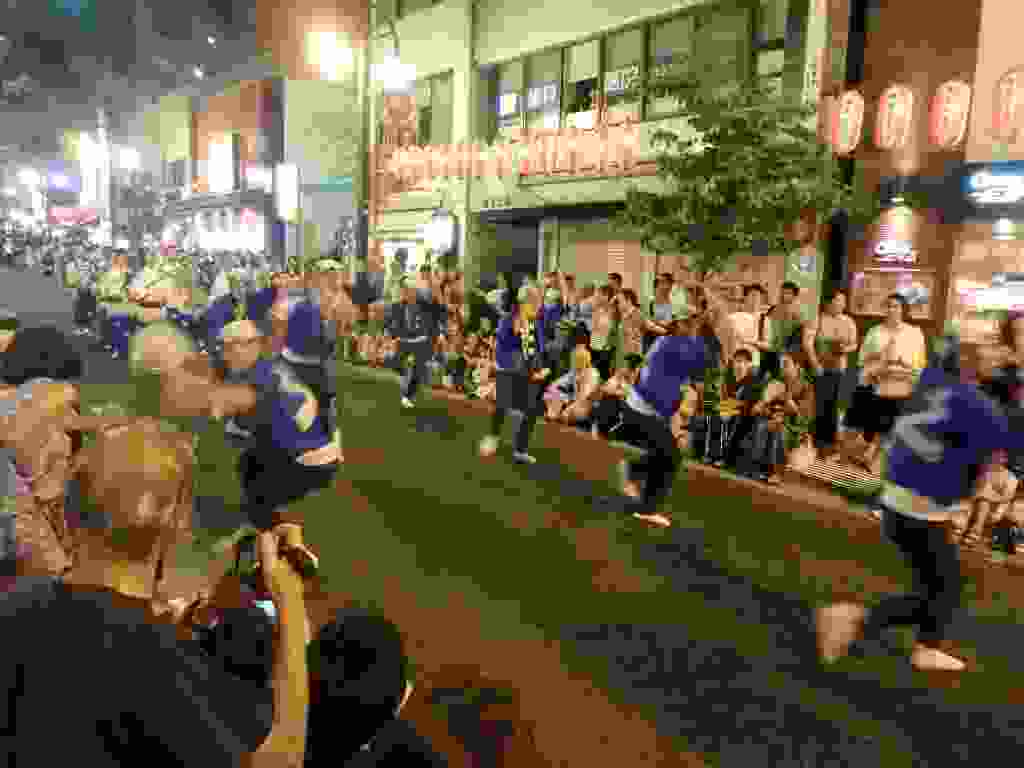
\includegraphics[width=\mywidth]{../wp-content/uploads/2015/07/P7245607-1024x768.jpg} \end{center}

 

 Repas dans un petit restaurant japonais, des spécialités originales et du saké : pas très fort et bon, ça ne ressemblait pas à ce que j'avais goûté en France. 

 

\begin{center} 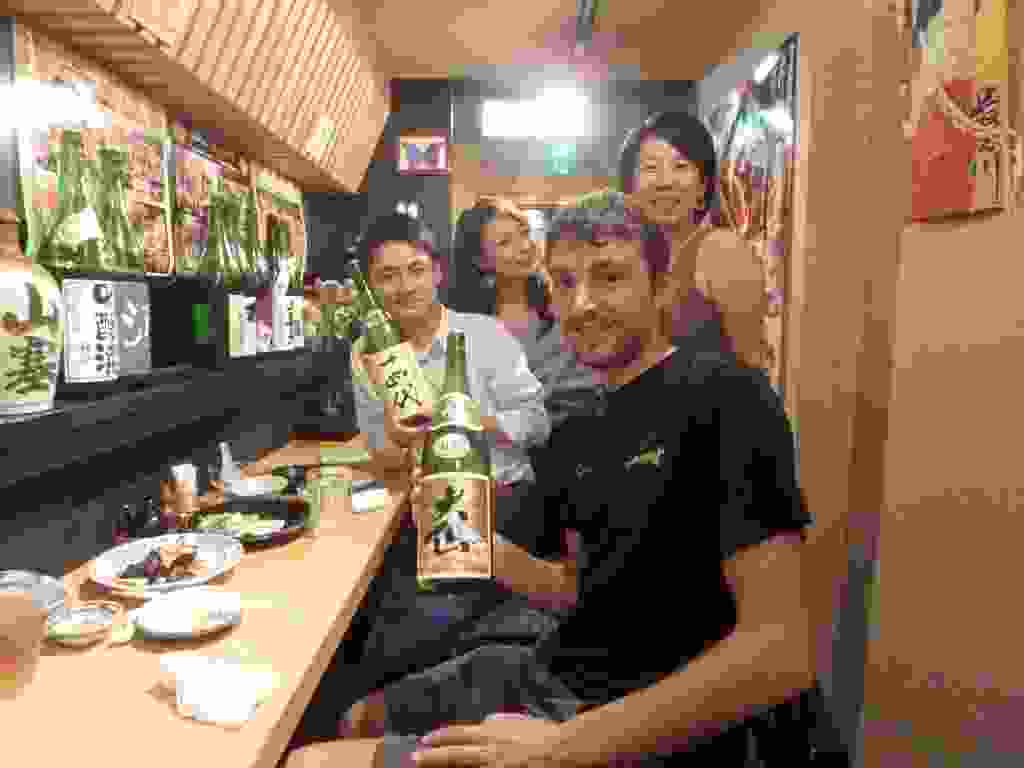
\includegraphics[width=\mywidth]{../wp-content/uploads/2015/07/P7245622-1024x768.jpg} \end{center}

 

 Quelques curiosités japonaises pour finir. 

 Toilettes high-tech 

 

\begin{center} 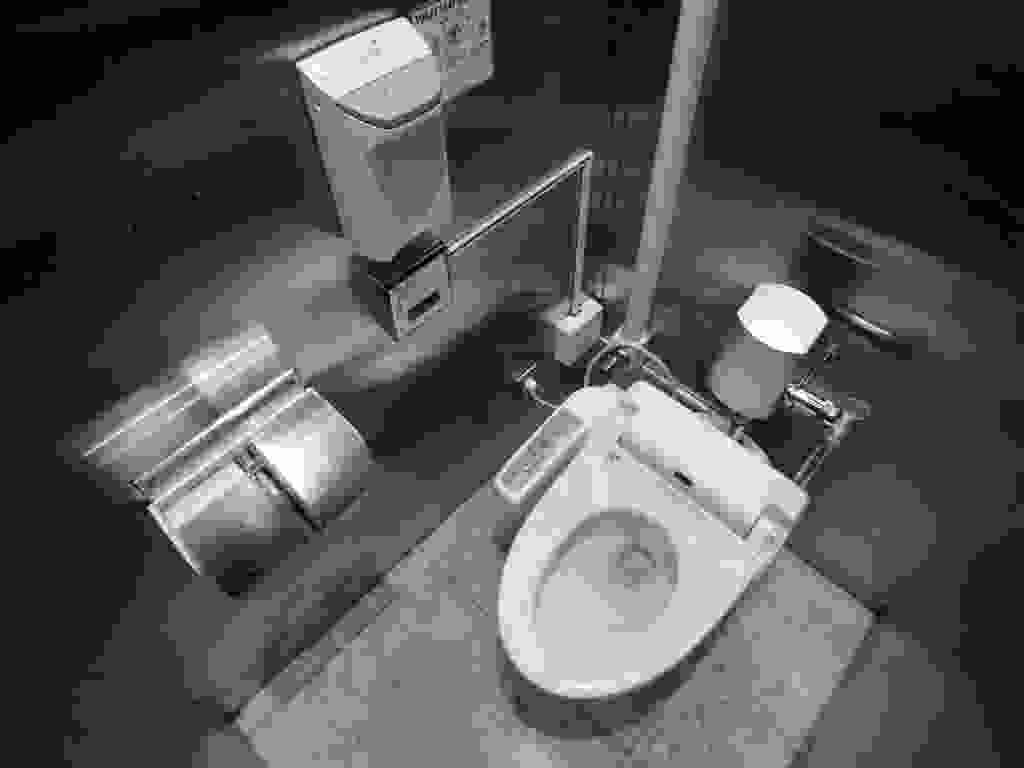
\includegraphics[width=\mywidth]{../wp-content/uploads/2015/07/OI000004-1024x768.jpg} \end{center}

 

 Les «convenience stores» quasiment à tous les coins de rues, ils font supermarchés, plats préparés, café, distributeur d'argent, journaux, tabac, toilettes… 

 

\begin{center} 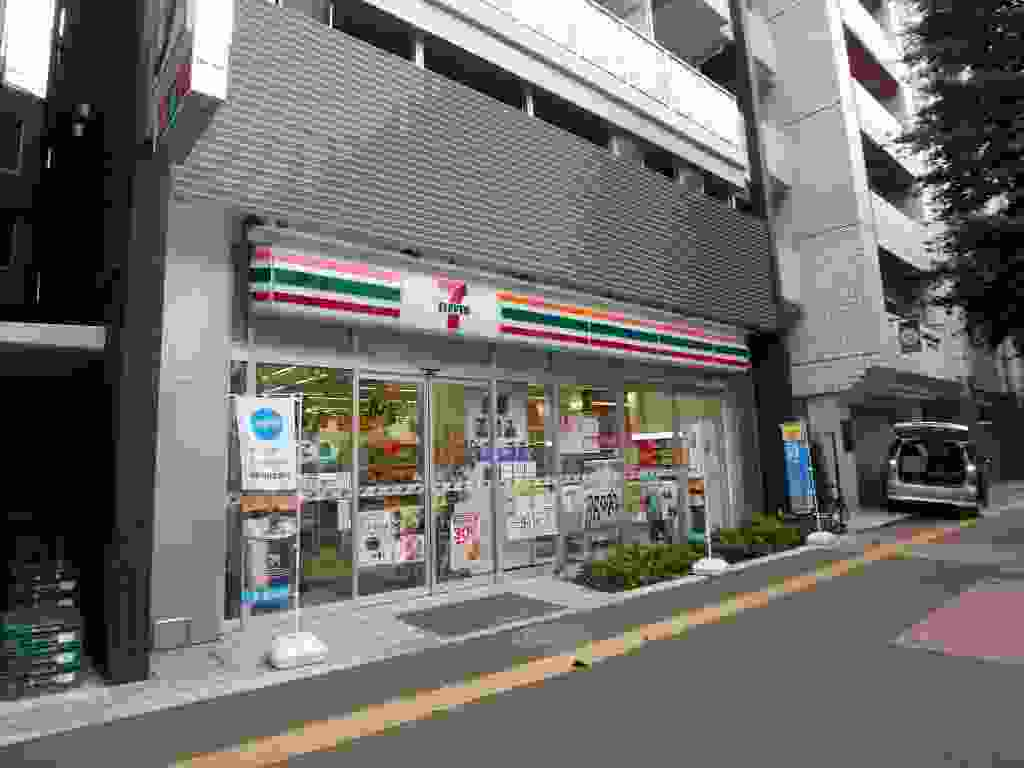
\includegraphics[width=\mywidth]{../wp-content/uploads/2015/07/P7195488-1024x768.jpg} \end{center}

 

 Vitrine de restaurant avec des reproduction des plats, pratique pour choisir. 

 

\begin{center} 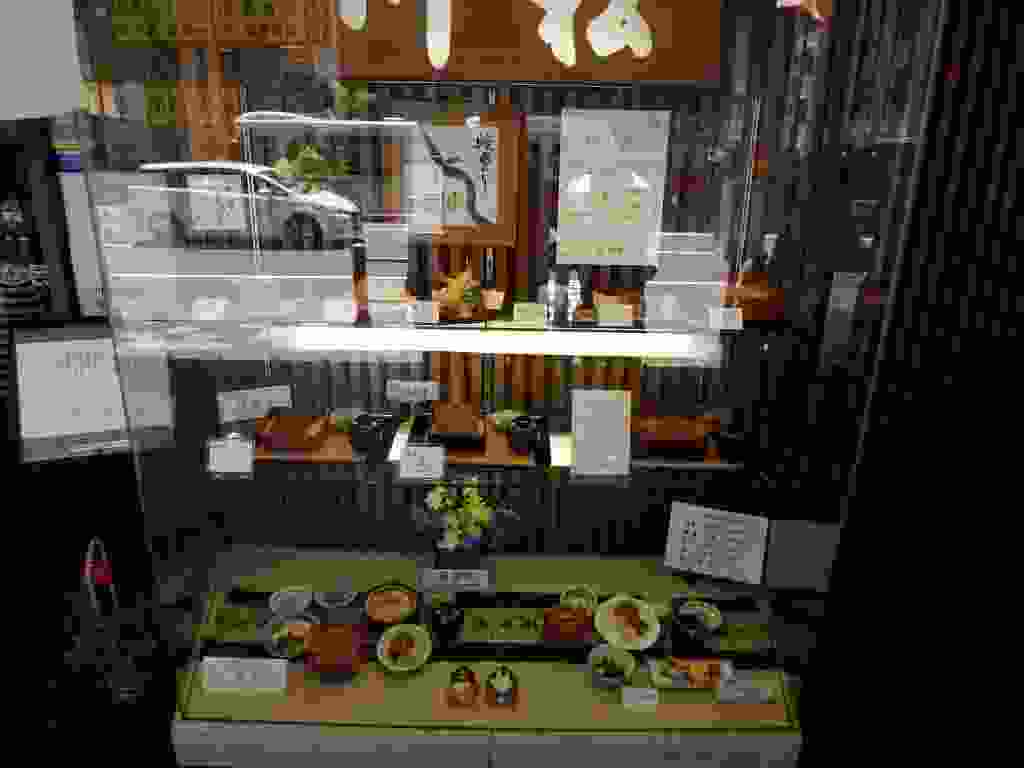
\includegraphics[width=\mywidth]{../wp-content/uploads/2015/07/P7195471-1024x768.jpg} \end{center}




 
 
